\lipsum[1-3]

%%!!!!!!!!!!!!!!!!!!!!!!!!!!!!!!!!!!!!!!!!!!!!!!!!!!!!!!!!!!!!!!!!!!!!!!!!!!!!!!
%%%%%%%%%%%%%%%%%%%%%%%%%%%%%%%%%%%%%%%%%%%%%%%%%%%%%%%%%%%%%%%%%%%%%%%%%%%%%%%%
%% SECTION: Przygotowanie eksperymentu
%%%%%%%%%%%%%%%%%%%%%%%%%%%%%%%%%%%%%%%%%%%%%%%%%%%%%%%%%%%%%%%%%%%%%%%%%%%%%%%%
%%!!!!!!!!!!!!!!!!!!!!!!!!!!!!!!!!!!!!!!!!!!!!!!!!!!!!!!!!!!!!!!!!!!!!!!!!!!!!!!
\section{Przygotowanie eksperymentu}

Eksperymentalna część pracy bezsprzecznie wymaga przygotowania odpowiedniego zestawu
sprzętu i~narzędzi. Konieczne jest wybranie odpowiedniej platformy sprzętowej
wspierającej komunikację bezprzewodową Bluetooth Low Energy w wersji minimum 5.0.
Niezbędne jest również oprzyrządowanie pomiarowe, które umożliwia pomiar natężeń
prądu poniżej 1mA, ze względu na energooszczędność urządzeń \gls{BLE}.

% zakładam, że we wcześniejszych rozdziałach definiuję zakres pracy i rodzaje eksperymentów

Badania zużycia energii wymagają aparatury, która w pełni zarejestruje minima i maksima
poboru prądu przy niskich błędach pomiarowych.

Eksperyment \gls{PER} wymaga przygotowania wielu zestawów uruchomieniowych obsługujących
komunikację BLE w konfiguracji Mesh. Dodatkowo, wymagane jest stworzenie dedykowanego oprogramowania
na mikrokontroler jak i komputer osobisty. Jest to niezbędne w celu kontroli przepływu
doświadczenia jak i akwizycji danych.

Niniejszy rozdział omawia zakres przygotowań do przeprowadzenia właściwych eksperymentów.


%%%%%%%%%%%%%%%%%%%%%%%%%%%%%%%%%%%%%%%%%%%%%%%%%%%%%%%%%%%%%%%%%%%%%%%%%%%%%%%%
%% SUBSECTION: Sprzęt i oprzyrządowanie
%%%%%%%%%%%%%%%%%%%%%%%%%%%%%%%%%%%%%%%%%%%%%%%%%%%%%%%%%%%%%%%%%%%%%%%%%%%%%%%%
\subsection{Sprzęt i oprzyrządowanie}

% nie pisać i tłumaczyć własnych preferencji. Raczej pisać generyczny bullshit

Próby doświadczalne oparto o produkty firmy ST. Decyzja podjęta została w oparciu
o osobiste preferencje autora pracy.

\subsubsection{P-NUCLEO-WB55}

Badania Bluetooth Low Energy wymagały wyboru platformy, która umożliwia eksperymentalną 
weryfikację wybranych celów badawczych. Ostatecznie, zdecydowano się na wykorzystanie 
mikrokontrolera \textit{STM32WB55RG}. W celu zapewnienia powtarzalności eksperymentu jak 
i~ze względu na ograniczenia czasowe, docelową platformą badawczą stał się zestaw 
uruchomieniowy \textit{P-NUCLEO-WB55}~\cite{noauthor_p-nucleo-wb55_nodate}.

\begin{figure}[!htb]
	\centering 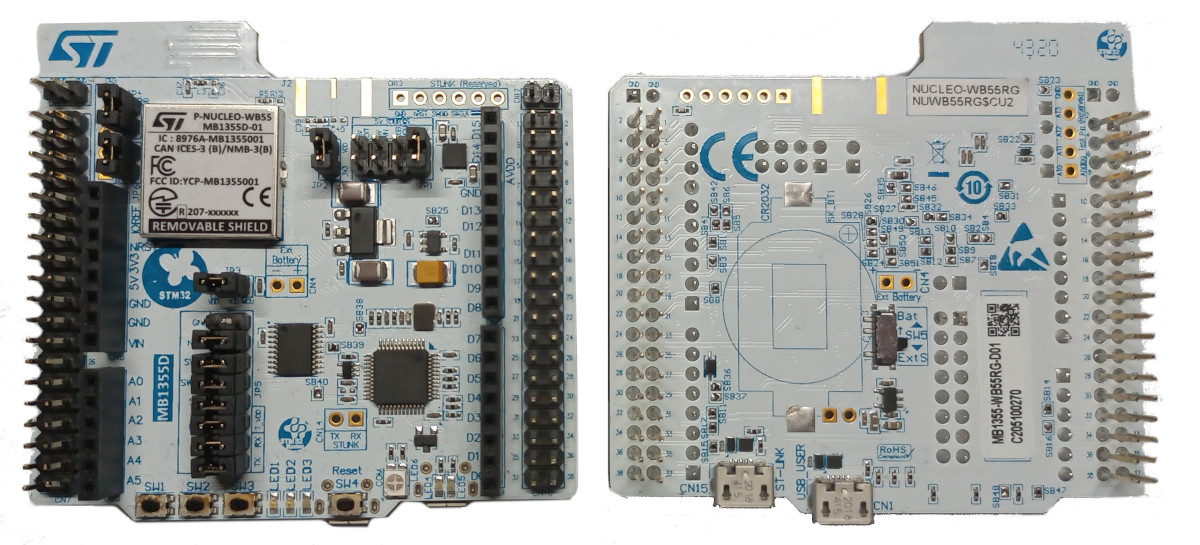
\includegraphics[width=0.618\linewidth]{nucleo_wb55.jpg}
	\caption{Zestaw uruchomieniowy P-NUCLEO-WB55}
	\label{rys:nucleo_wb55}
\end{figure}

Zestaw ten zgodny jest ze specyfikacją Bluetooth Low Energy v5.0. Dodatkowo, wspiera
on inne standardy komunikacji, m.in. Zigbee~\cite{noauthor_stm32wb_2022}.
Ten fakt może zostać wykorzystany w celu bezpośredniego porównania różnych stosów komunikacji bezprzewodowej.
Nie jest to jednak celem niniejszej pracy, a stanowi możliwość jej dalszego 
rozwinięcia.


\subsubsection{X-NUCLEO-LPM01A} \label{device:plytka_pomiarowa}

Płytka rozszerzeń X-NUCLEO-LPM01A spełnia wszelkie oczekiwania dotyczące możliwości pomiarowych
stawianych przed projektem. Wg oficjalnej dokumentacji \cite{noauthor_um2243_2018}, układ oferuje:

\begin{itemize}
\item Programowalne źródło napięciowe 1,8V do 3,3V
\item Dynamiczne próbkowanie w zakresie od 100nA 50mA przy maksymalnej częstotliwości 100kHz z 2\%-ową dokładnością pomiarów
\item Pomiar statyczny natężenia prądu do 200mA
\item Integracja z aplikacją do dedykowaną aplikacją akwizycji danych \cite{noauthor_stm32cubemonpwr_2022}
\end{itemize}

\begin{figure}[!ht]
	\centering 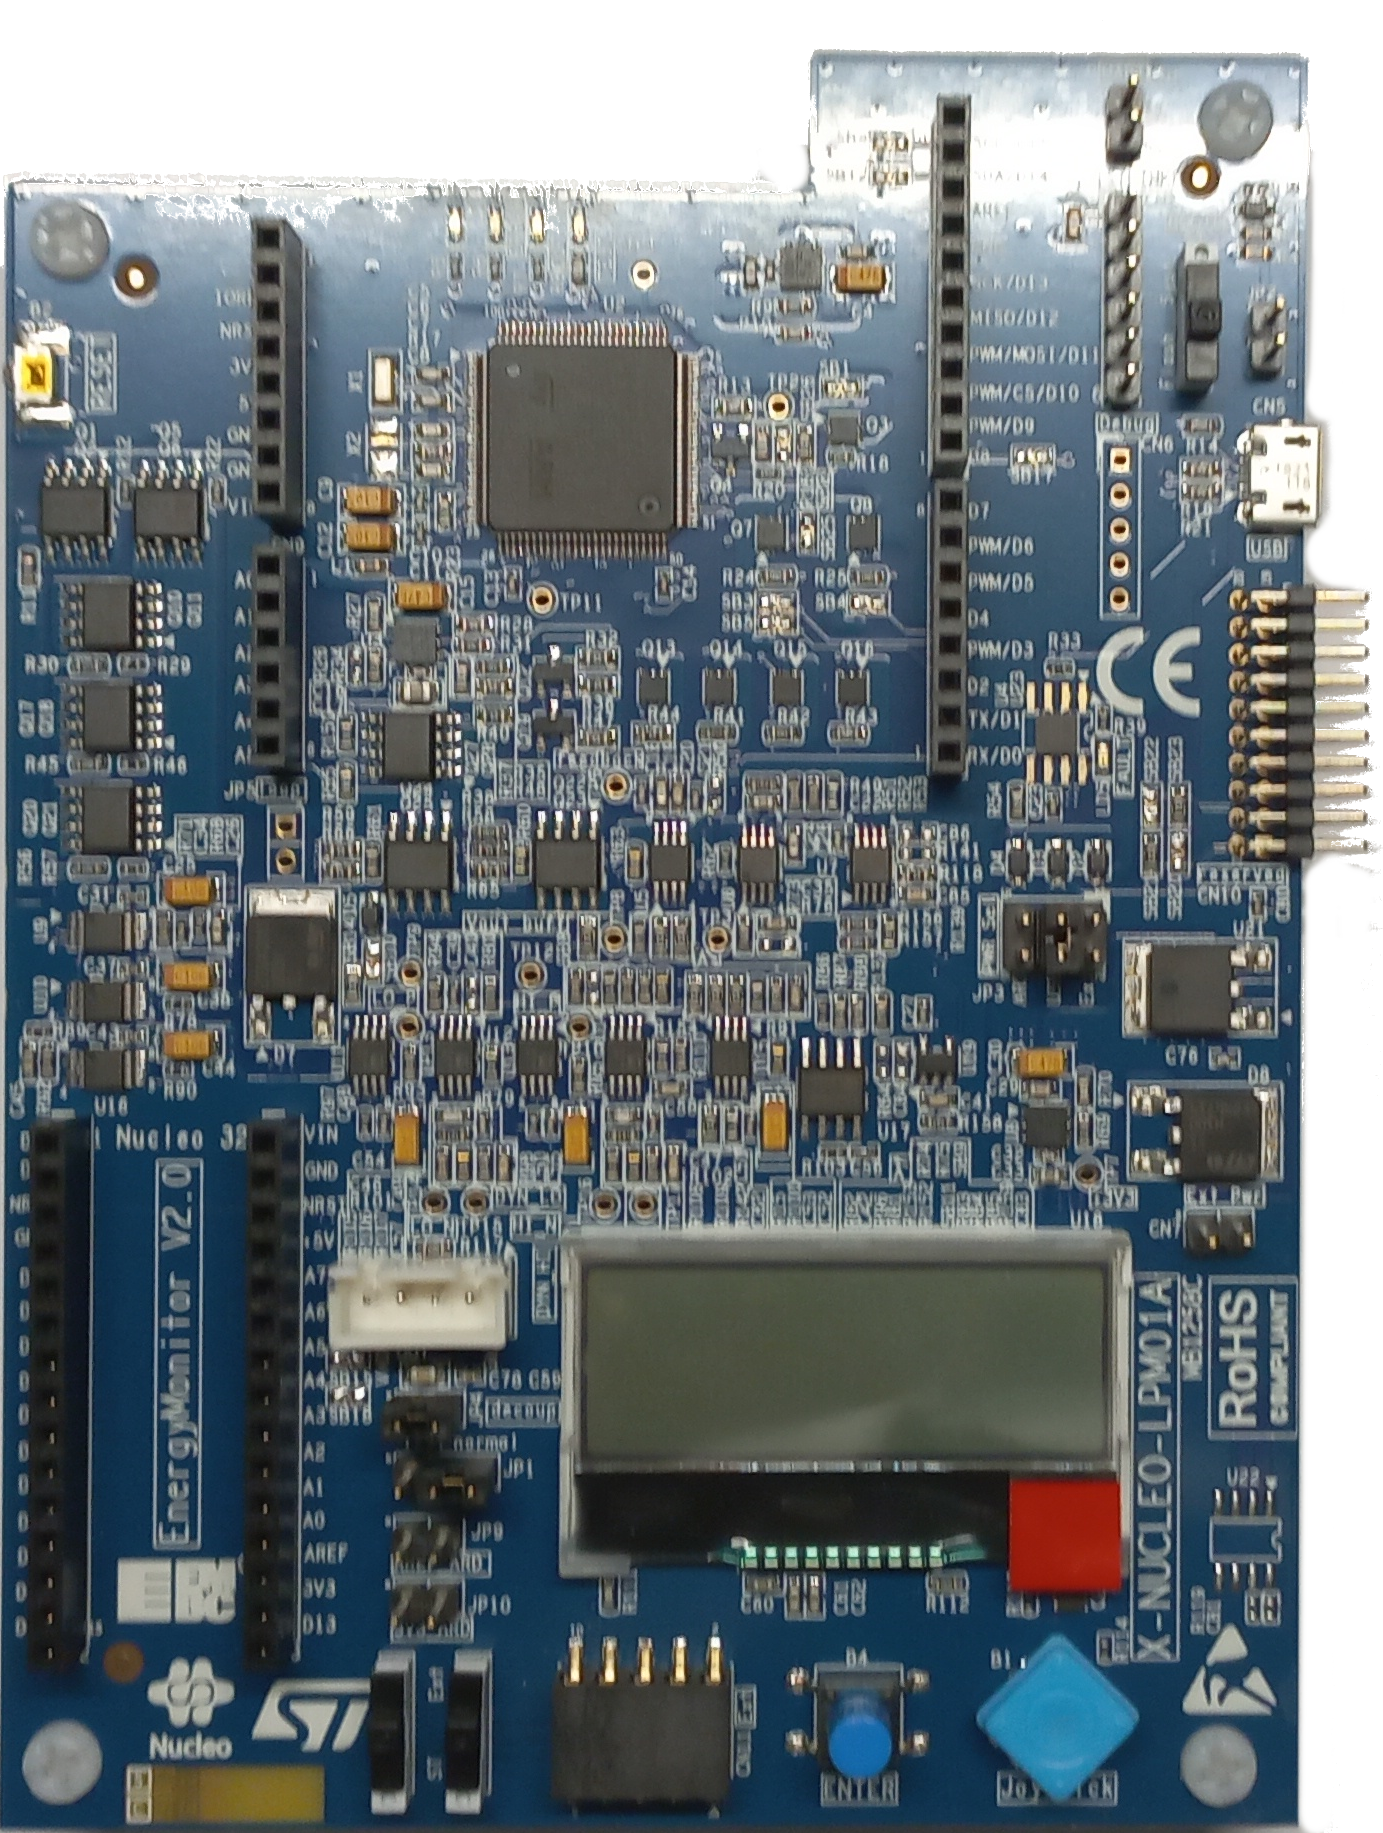
\includegraphics[width=0.618\linewidth]{st_power_measurement_unit.png}
	\caption{Zestaw pomiarowy X-NUCLEO-LPM01A}
	\label{rys:nucleo_lpm01a}
\end{figure}

Moduł ten nie ogranicza się tylko do wykorzystywania autorskich złącz firmy ST. Schemat wyprowadzeń pinów
umożliwia wykorzystanie popularnych platform takich jak Arduino\footnote{https://www.arduino.cc/}. Co istotniejsze, wybrana płytka umożliwia
zasilanie dowolnego układu dzięki wyprowadzeniu źródła napięciowego za pośrednictwem pinów 
(za dokumentacją: złącze CN14). Ten fakt został wykorzystany w badaniach, pozwalając uniknąć kłopotliwej
konfiguracji P-NUCLEO-WB55 wymagającej tworzenia dodatkowych ścieżek lutowanych.

Dodatkową cechą tego modułu jest akwizycja danych z użyciem komputera osobistego. Dzięki dedykowanej
aplikacji, dostarczanej wraz z modułem, możliwa jest akwizycja danych w czasie rzeczywistym przy
wybranych częstotliwościach próbkowania. Zebrane w ten sposób dane służą dalszym analizom, co zostało
wykorzystane w niniejszej pracy. 

\subsubsection{Narzędzia i firmware firmy ST}
Firma ST wraz z zestawem uruchomieniowym udostępnia pełne zintegrowane środowisko
programistyczne oraz niezbędne biblioteki i certyfikowany firmware:

\begin{itemize}
\item \textbf{STM32CubeIDE} \cite{noauthor_stm32cubeide_2022} - multiplatformowe zintegrowane środowisko programistyczne
dostarczane przez ST bazujące na otwartoźródłowym środowisko \textit{Eclipse}\footnote{https://www.eclipse.org/ide/}.
\item \textbf{STM32CubeProgrammer} \cite{noauthor_stm32cubeprog_2022} - narzędzie umożliwiające wykonywanie operacji
odczytu, zapisu i weryfikacji skompilowanego oprogramowania produktów STM32. 
\item \textbf{STM32CubeMonitor-Power} \cite{noauthor_stm32cubemonpwr_2022} - oprogramowanie służące akwizycji danych
o zużyciu energii m.in. w zestawie X-NUCLEO-LPM01A Rysunek: \ref{rys:nucleo_lpm01a}.
\item \textbf{Firmware STM32CubeWB} \cite{noauthor_stm32cubewb_2022} - zestaw bibliotek, narzędzi oraz przykładów
przeznaczonych dla mikrokontrolerów rodziny STM32WB. W skład tego repozytorium wchodzą zależności takie jak:
skompilowany, zamknięty firmware ko-processora dla różnych stosów połączeń bezprzewodowych; przykłady programów
wykorzystujące biblioteki HAL jak i również bezpośrednio rejestry; przykłady BLE; przykłady BLE Mesh.
\end{itemize}

%%%%%%%%%%%%%%%%%%%%%%%%%%%%%%%%%%%%%%%%%%%%%%%%%%%%%%%%%%%%%%%%%%%%%%%%%%%%%%%%
%% SUBSECTION: Zasilanie i obudowy
%%%%%%%%%%%%%%%%%%%%%%%%%%%%%%%%%%%%%%%%%%%%%%%%%%%%%%%%%%%%%%%%%%%%%%%%%%%%%%%%
\subsection{Narzędzia i elementy dodatkowe}

\subsubsection{Zasilanie}
Próby terenowe wymagają odrębnego, właściwego zasilania. Wybrane zestawy uruchomieniowe
wykorzystują ustandaryzowane złącze komunikacyjne USB. Złącze to oprócz komunikacji
oferuje zasilanie linią +5V. Przeprowadzając właściwe eksperymenty wykorzystano
komercyjnie dostępne banki energii tzw. powerbanki. Są to akumulatory litowo-jonowe
lub litowo-polimerowe z wbudowanym systemem zarządzania baterią\footnote{\gls{BMS} - ang. Battery Management System}
i właściwymi przetwornicami impulsowymi w celu zapewnienia odpowiedniego napięcia zasilania.

Elektronika wbudowane w magazyny energii automatycznie wyłącza zasilanie w przypadku braku
podłączonego urządzenia lub gdy dane urządzenie pobiera marginalnie niskie wartości
prądu. Służy to ochronie cennego i delikatnego akumulatora. Jest to cecha korzystna
z punktu widzenia konsumenta kupującego powerbank w celu szybkiego ładowania urządzeń elektronicznych.
Niestety, zaleta ta staje się wadą w przypadku przeprowadzanych doświadczeń. Podłączając moduł P-NUCLEO-WB55,
urządzenie po pewnym okresie działania wyłącza się na skutek uruchomionych zabezpieczeń w źródle energii.

W celu skonstruowano trywialne urządzenie, które wlutowane równolegle w linię zasilania 5V,
konsumuje ok. 100mA prądu: $0,5W = 5V \cdot 0,02A \cdot 5 [diod]$. Doświadczalnie stwierdzono, że tak włączony
odbiornik energii umożliwia stabilne działanie włączonego do sieci modułu STM32. Schemat 
zaprezentowano na Rysunku~\ref{rys:power_led_consumer}

\begin{figure}[!ht]
	\centering 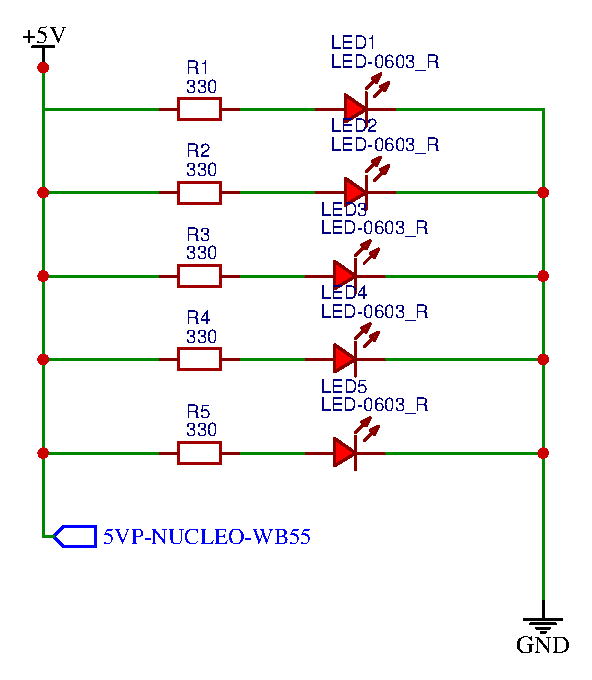
\includegraphics[width=0.618\linewidth]{power_led_consumer.pdf}
	\caption{Odbiornik energii}
	\label{rys:power_led_consumer}
\end{figure}

\subsubsection{Obudowa - druk 3D}
Kolejnym elementem niezbędnym w celu przeprowadzenia eksperymentów terenowych jest zapewnienie
ochrony mechanicznej wybranych zestawów uruchomieniowych. Podczas prób elementy mogą zostać
fizycznie uszkodzone poprzez m.in. wyłamanie fragmentu \gls{PCB} (w~tym anteny), uszkodzenie pinów etc.

Wykorzystując techniki projektowania wspomaganego komputerowo\footnote{\gls{CAD} - ang. \textit{Computer-aided Design}},
zaprojektowano autorską obudowę. Głównym celem projektowym było zapewnienie minimalnej ochrony
mechanicznej, jednocześnie redukując możliwy wpływ materiału na tłumienie sygnału. Elementy
interfejsu: przyciski i~antena, zostały celowo wyeksponowane. Rzut izometryczny przedstawiony został
na Rysunku~\ref{rys:obudowa_model3d}.


\begin{figure}[!htb]
	\centering 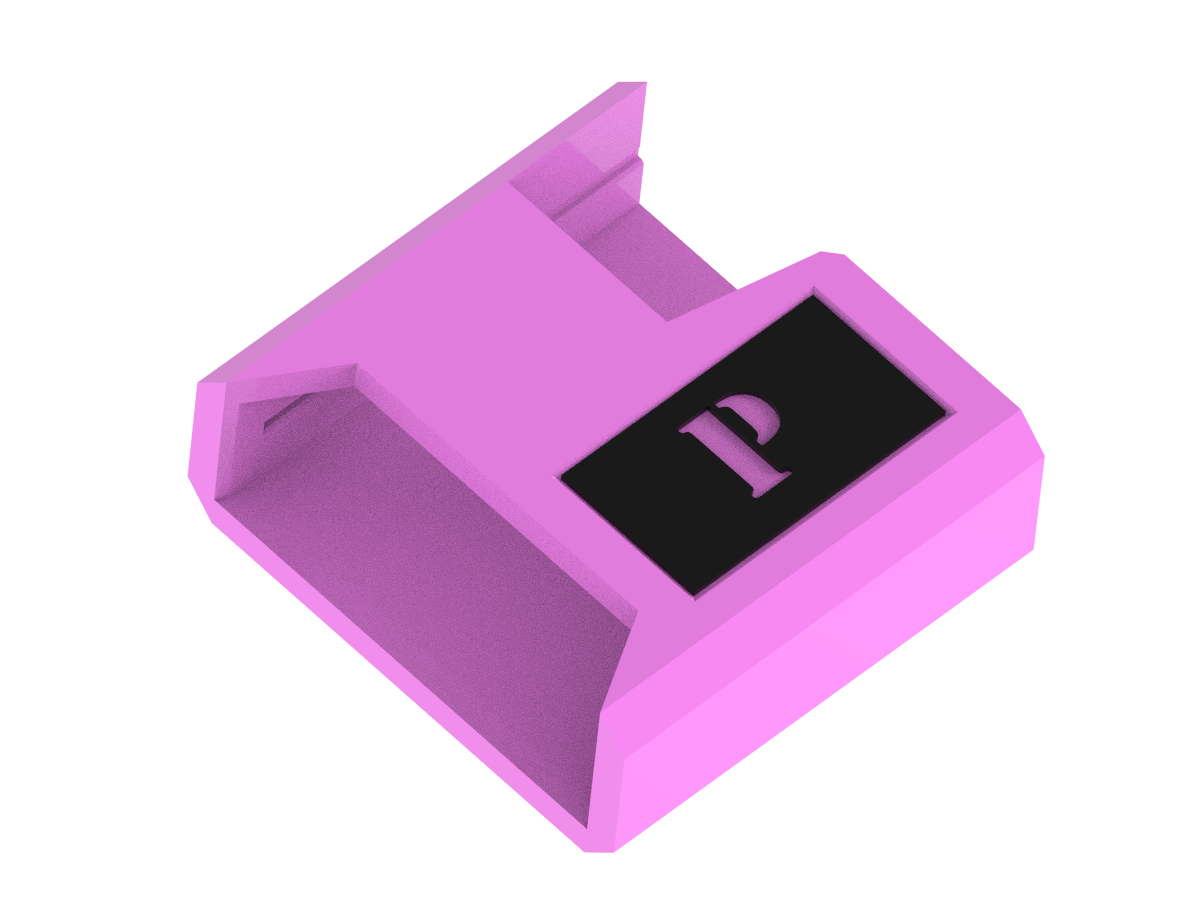
\includegraphics[width=0.618\linewidth]{stm_case_render.png}
	\caption{Model obudowy dla zestawu P-NUCLEO-WB55}
	\label{rys:obudowa_model3d}
\end{figure}

Obudowa wykonana została z materiału \gls{PLA}\footnote{PLA - ang. \textit{Polylactic acid}, polilaktyd} techniką
druku 3D \gls{FDM}\footnote{FDM - ang. \textit{Fused Deposition Modeling}}/\gls{FFF}\footnote{FFF - \textit{Fused Filament Fabrication}}.
Jednobryłowa konstrukcja podyktowana została chęcią uproszczenia wydruku, kosztem zwiększonych trudności
doboru tolerancji dla umieszczanych wewnątrz płytek \gls{PCB}. Obudowa przewiduje wsuwanie modułu Nucleo
do wewnątrz, zapewniając jednoczesne pewne jego mocowanie.

Dobór koloru wydruku również nie był przypadkowy. Przewidując potencjalne lokalizacje przeprowadzanych
doświadczeń, wybrano kolor możliwie jaskrawy. Podstawowym założeniem było ułatwienie dostrzeżenia
obudowy, a wraz z obudową również zestawu uruchomieniowego, pośród flory leśnej czy terenów
zurbanizowanych. Ostateczne wykonanie obudów zaprezentowano na Rysunku~\ref{rys:obudowa_wykonanie}.

\begin{figure}[!htb]
	\centering 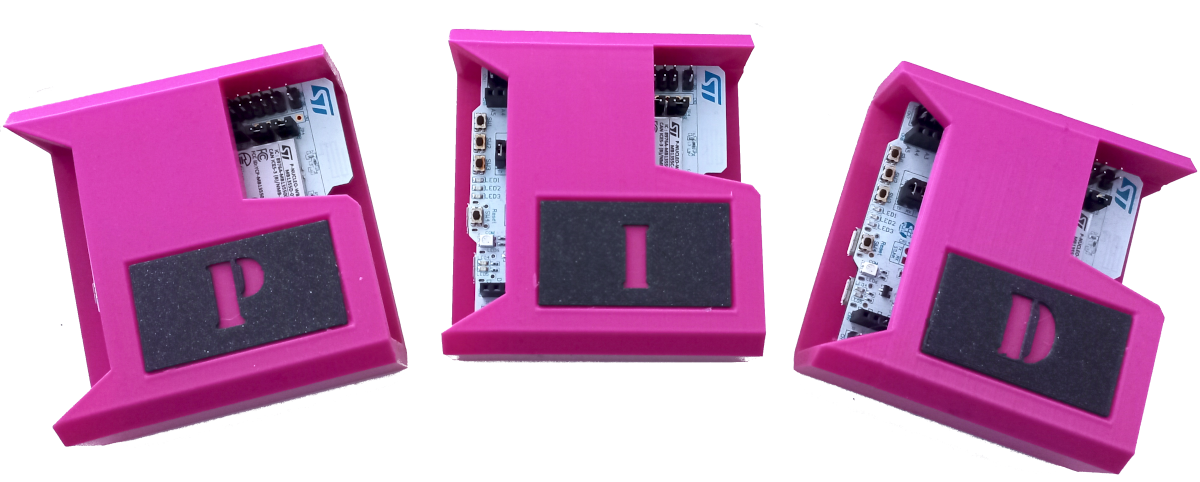
\includegraphics[width=0.618\linewidth]{3d_real_cases.png}
	\caption{Obudowa zestawu uruchomieniowego Nucleo wykonana w technologii druku 3D - realizacja}
	\label{rys:obudowa_wykonanie}
\end{figure}

%%%%%%%%%%%%%%%%%%%%%%%%%%%%%%%%%%%%%%%%%%%%%%%%%%%%%%%%%%%%%%%%%%%%%%%%%%%%%%%%
%% SUBSECTION: Oprogramowanie mikrokontrolera
%%%%%%%%%%%%%%%%%%%%%%%%%%%%%%%%%%%%%%%%%%%%%%%%%%%%%%%%%%%%%%%%%%%%%%%%%%%%%%%%
\subsection{Oprogramowanie mikrokontrolera} \label{prep:uc-software}

\begin{lstlisting}[language=C,
    caption={Testowy kod C},
    label={lst:kod cpp}]
MOBLE_RESULT Appli_Generic_OnOff_Set(Generic_OnOffStatus_t* pGeneric_OnOffParam, 
                                     MOBLEUINT8 OptionalValid,
                                     MOBLEUINT16 dstPeer,
                                     MOBLEUINT8 elementIndex)
{
  /* LED control only for main element */
  if(elementIndex == GENERIC_SERVER_MAIN_ELEMENT_INDEX)
  {
  // [...]
      if(AppliOnOffSet[elementIndex].Present_OnOffValue == AppliOnOffSet[elementIndex].TargetValue)
      {
    	if (dstPeer != 0xc000) {
    	   increment_generic_onoff_counter_packet_error_rate_experiment(AppliOnOffSet[elementIndex].Present_OnOffValue, dstPeer);
    	}
        if(AppliOnOffSet[elementIndex].Present_OnOffValue > 0)
        {
          BSP_LED_On(LED_BLUE);
        }
        else
        {
          BSP_LED_Off(LED_BLUE);
        }
      }
    }  
  // [...]
\end{lstlisting}

%%%%%%%%%%%%%%%%%%%%%%%%%%%%%%%%%%%%%%%%%%%%%%%%%%%%%%%%%%%%%%%%%%%%%%%%%%%%%%%%
%% SUBSECTION: Oprogramowanie PC
%%%%%%%%%%%%%%%%%%%%%%%%%%%%%%%%%%%%%%%%%%%%%%%%%%%%%%%%%%%%%%%%%%%%%%%%%%%%%%%%
\subsection{Oprogramowanie PC} \label{prep:pc-software}


%%!!!!!!!!!!!!!!!!!!!!!!!!!!!!!!!!!!!!!!!!!!!!!!!!!!!!!!!!!!!!!!!!!!!!!!!!!!!!!!
%%%%%%%%%%%%%%%%%%%%%%%%%%%%%%%%%%%%%%%%%%%%%%%%%%%%%%%%%%%%%%%%%%%%%%%%%%%%%%%%
%% SECTION: Zużycie energii
%%%%%%%%%%%%%%%%%%%%%%%%%%%%%%%%%%%%%%%%%%%%%%%%%%%%%%%%%%%%%%%%%%%%%%%%%%%%%%%%
%%!!!!!!!!!!!!!!!!!!!!!!!!!!!!!!!!!!!!!!!!!!!!!!!!!!!!!!!!!!!!!!!!!!!!!!!!!!!!!!
\section{Zużycie energii}

%%%%%%%%%%%%%%%%%%%%%%%%%%%%%%%%%%%%%%%%%%%%%%%%%%%%%%%%%%%%%%%%%%%%%%%%%%%%%%%%
%% SUBSECTION: Metodologia badania
%%%%%%%%%%%%%%%%%%%%%%%%%%%%%%%%%%%%%%%%%%%%%%%%%%%%%%%%%%%%%%%%%%%%%%%%%%%%%%%%
\subsection{Metodologia badania}

Podstawą badania zużycia energii jest pomiar wartości pobieranego prądu przez zestaw uruchomieniowy
P-NUCLEO-WB55 w czasie. Posiadając dane wymienione dane, na podstawie oczywistych
zależności fizycznych wyznacza się parametry jak całkowita wykorzystana energia
podczas badania, przedstawiona w przystępnej postaci parametru mocy.

Pomiary wartości chwilowego poboru prądu oparto o moduł opisany w punkcie~\ref{device:plytka_pomiarowa}.
Źródłem energii dla płytki pomiarowej jest komputer klasy PC, a precyzyjniej udostępniany
port USB. Wykorzystując również ten protokół następuje transmisja danych poprzez komunikację szeregową
UART, umożliwiając akwizycję danych.

Połączenie z zestawem uruchomieniowym oparto o konektor CN14 udostępniający piny: PIN1 - masa GND, PIN3 - VCC $3.3V$~\cite{noauthor_um2243_2018}.
Wyprowadzone przewody połączono następnie z P-NUCLEO-WB55 poprzez konektor JP2, wcześniej pozbawiony zawleczki.
Jest to metoda rekomendowana dla pomiaru prądu opisana w dokumentacji zestawu~\cite{stmicroelectronics_um2435_2019}\footnote{
Rozdział 7.12 Current measurement}. Porty kompatybilne z Arduino/ST Morpho mogłyby stanowić równorzędny sposób
włączenia zestawu uruchomieniowego do obwodu płytki pomiarowej. Autorska analiza dokumentacji sugeruje jednak,
iż opcja ta nie jest wspierana. Wymagane byłoby lutowanie dodatkowego połączenia w (punkcie SB27), by móc wykorzystać
zasilanie napięciem $3.3V$.

\begin{figure}[!htb]
	\centering 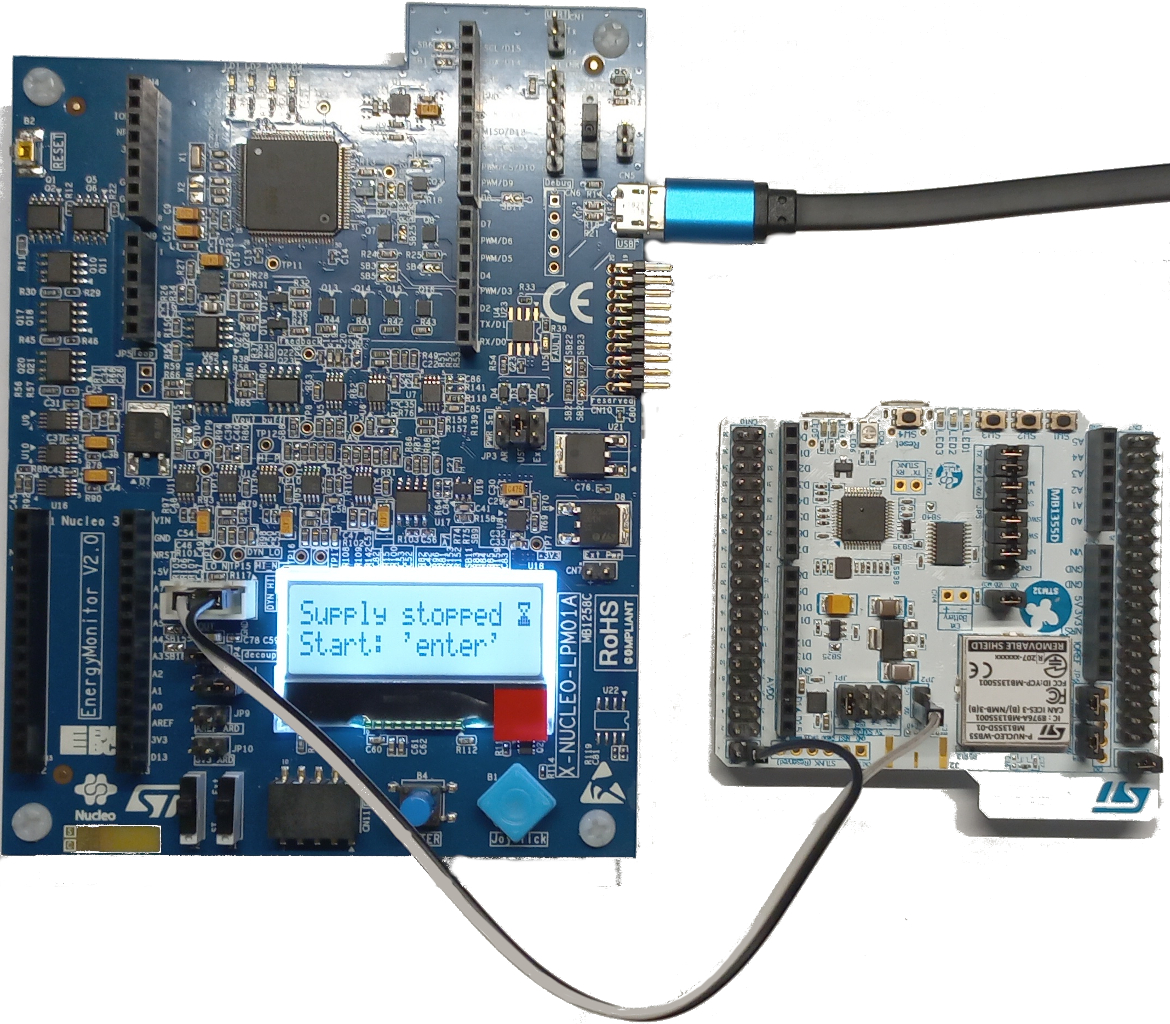
\includegraphics[width=0.618\linewidth]{power_measurement_unit_connected.png}
	\caption{Podłączony zestaw pomiarowy}
	\label{rys:connected_power_measurement_unit}
\end{figure}

Celem akwizycji danych wybrano dostarczane przez producenta oprogramowanie \textit{STM32CubeMonitor-Power}.
Pojedyncza sesja pomiarowa trwająca 100 sekund zapewnia niezbędne dane. Są one następnie
odpowiednio przetwarzane poprzez odcięcie wartości zebranych w ostatnich sekundach. Związane to było
ze sposobem działania mikrokontrolera, który po 60 sekundach przechodzi w stan zwiększonej
oszczędności energii. Stąd, by rozróżnić różne tryby pracy \gls{BLE}, zdecydowano o odcięciu
połowy okresu pomiarowego, zapewniając jednolite wartości względem trybów zużycia energii
w~50 sekundowym oknie.

\begin{figure}[!htb]
	\centering 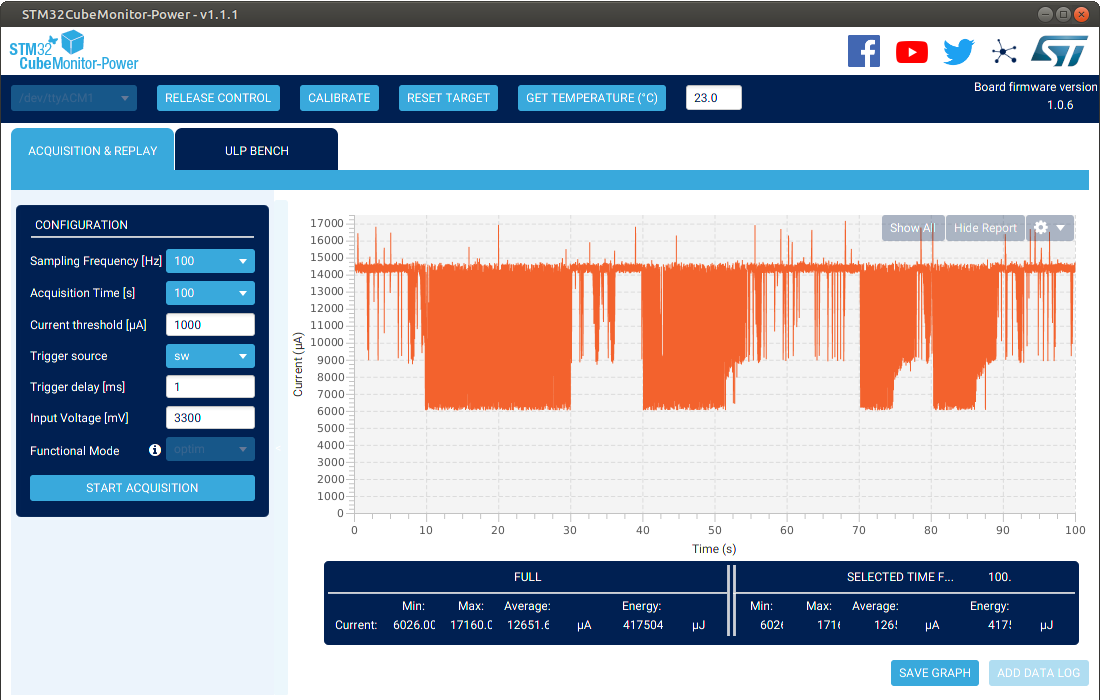
\includegraphics[width=0.99\linewidth]{stm32_power_monitor_sample.png}
	\caption{Przykładowa sesja pomiarowa dla BLE Mesh - sieć w trybie nasłuchującym}
	\label{rys:measurement_session_sample}
\end{figure}

Tak zebrane dane następnie przetworzono uzyskując wartości energii i średniej mocy
użytej przez układ. Wykorzystuje się w celu oczywistą zależność fizyczną zaprezentowaną
wzorem~\ref{energy_equation}\cite{skoro_marta_fizyka_1973}.

\begin{equation} \label{energy_equation}
E_{\text{całkowita}} = U \cdot \int_{t=0[s]}^{t=50[s]} \mathrm{d}i \: \mathrm{d} t
\end{equation}

\begin{equation} \label{power_equation}
P = \frac{E_{\text{całkowita}}}{t}
\end{equation}

gdzie:

\begin{description}
\item $E_{\text{całkowita}} [J]$ - wykorzystana energia podczas 50s sekundowej sesji rejestracji danych
\item $P [W]$ - moczużyta podczas 50s sekundowej sesji rejestracji danych
\item $U [V]$ - napięcie zasilania mikrokontrolera - 3.3V - stała
\item $\mathrm{d}i [A]$ - prąd w danej chwili
\item $\mathrm{d}t [s]$ - podstawa czasowa całkowania, 0.01s/interwał (100Hz) - stała 
\end{description}

Zebrane dane w postaci wartości chwilowych pobieranego przez mikrokontroler prądu względem czasu
przetworzono z użyciem metod numerycznych. W~celu wyliczenia łącznej wykorzystanej energii, a~tym samym
mocy, stosuje się zależność~\ref{energy_equation}. Uwzględniając fakt działania w domenie dyskretnej,
wykorzystano kompozytową metodę całkowania Simpsona~\cite{noauthor_scipyintegratesimpson_nodate}.
Podstawą dla całkowania są wartości zebrane w równoodległych odstępach. Dokonując akwizycji danych
dobrano częstotliwość próbkowania jako $100Hz$. Każda kolejna wartość charakteryzuje się więc
10 milisekundową różnicą w~podstawie czasu. Uwzględniając ten fakt, wyliczenie wartości
wykorzystanej energii jak i~mocy staje się trywialne.

%%%%%%%%%%%%%%%%%%%%%%%%%%%%%%%%%%%%%%%%%%%%%%%%%%%%%%%%%%%%%%%%%%%%%%%%%%%%%%%%
%% SUBSECTION: BT Low Energy - Usługa Heart Rate
%%%%%%%%%%%%%%%%%%%%%%%%%%%%%%%%%%%%%%%%%%%%%%%%%%%%%%%%%%%%%%%%%%%%%%%%%%%%%%%%
\subsection{BT Low Energy - Usługa Heart Rate}

\lipsum[1-3]
\begin{figure}[!htb]
	\centering 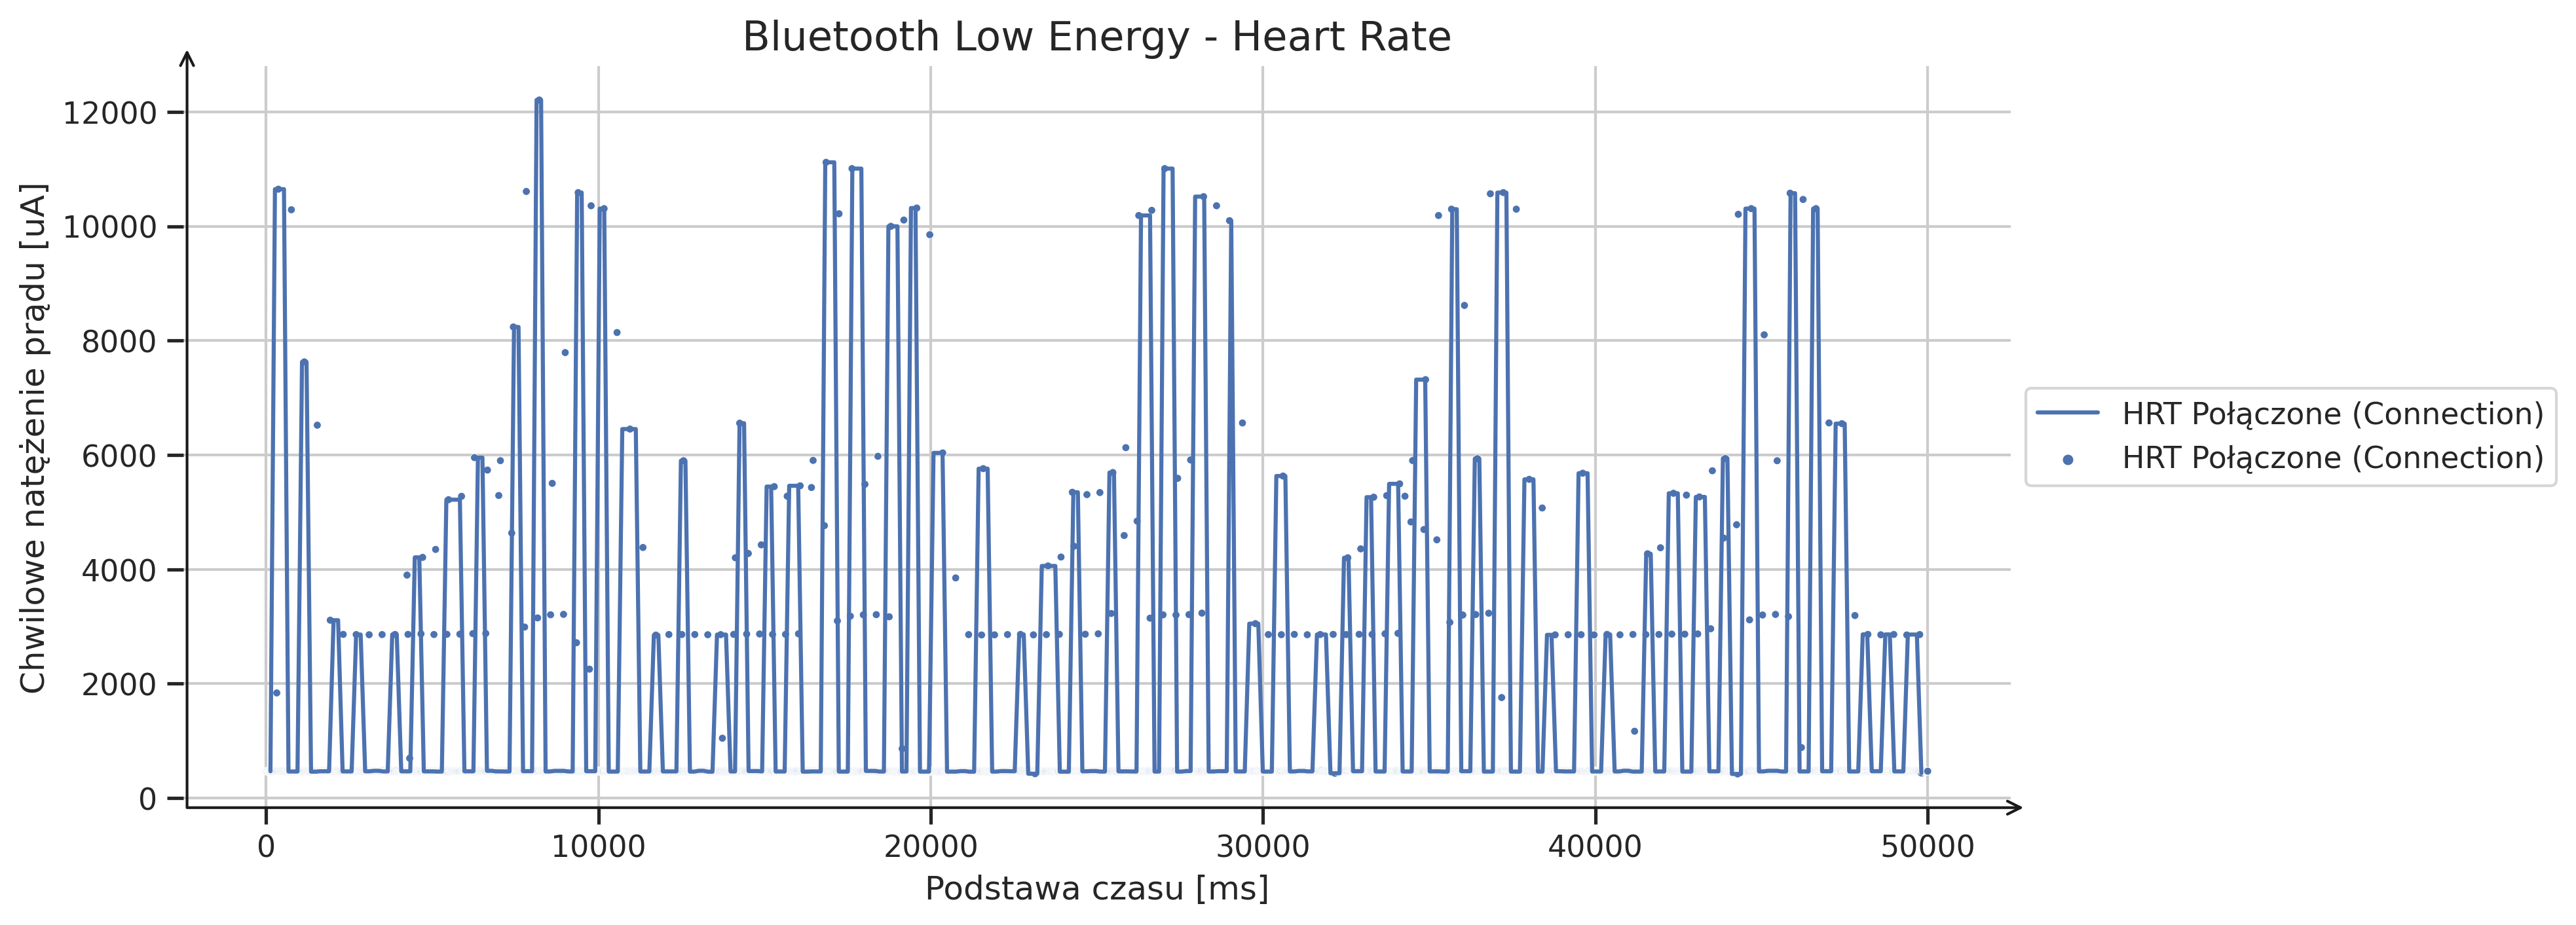
\includegraphics[width=0.99\linewidth]{power_ble_hr_connected_only_amps.png}
	\caption{Charakterystyka czasowa poboru prądu dla BLE i usługi Heart Rate - Usługa Połączona}
	\label{rys:power_ble_hr_connected_only_amps}
\end{figure}

\lipsum[1-3]
\begin{figure}[!htb]
	\centering 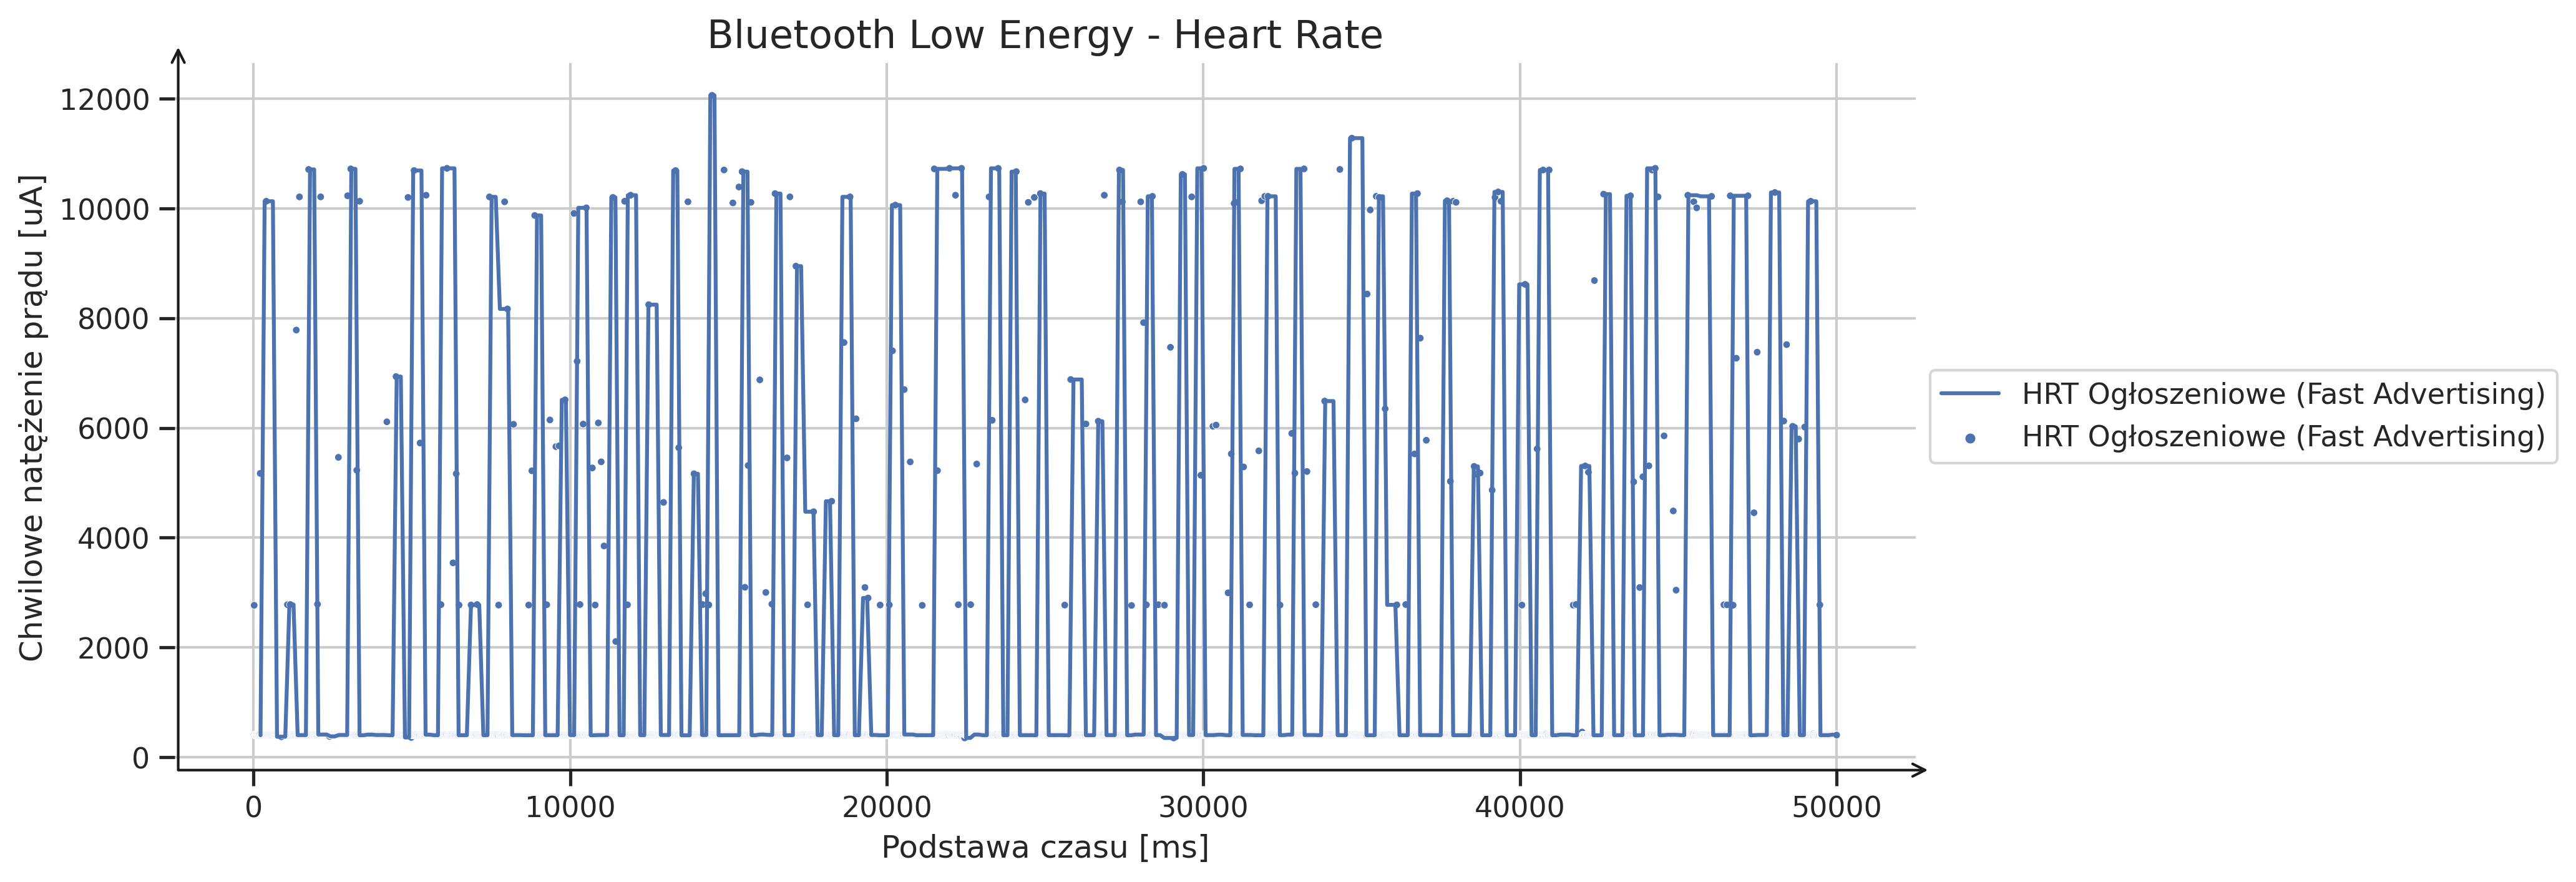
\includegraphics[width=0.99\linewidth]{power_ble_hr_fastadv_only_amps.png}
	\caption{Charakterystyka czasowa poboru prądu dla BLE i usługi Heart Rate - Tryb szybkiego ogłoszenia}
	\label{rys:power_ble_hr_fastadv_only_amps}
\end{figure}

\lipsum[1-3]
\begin{figure}[!htb]
	\centering 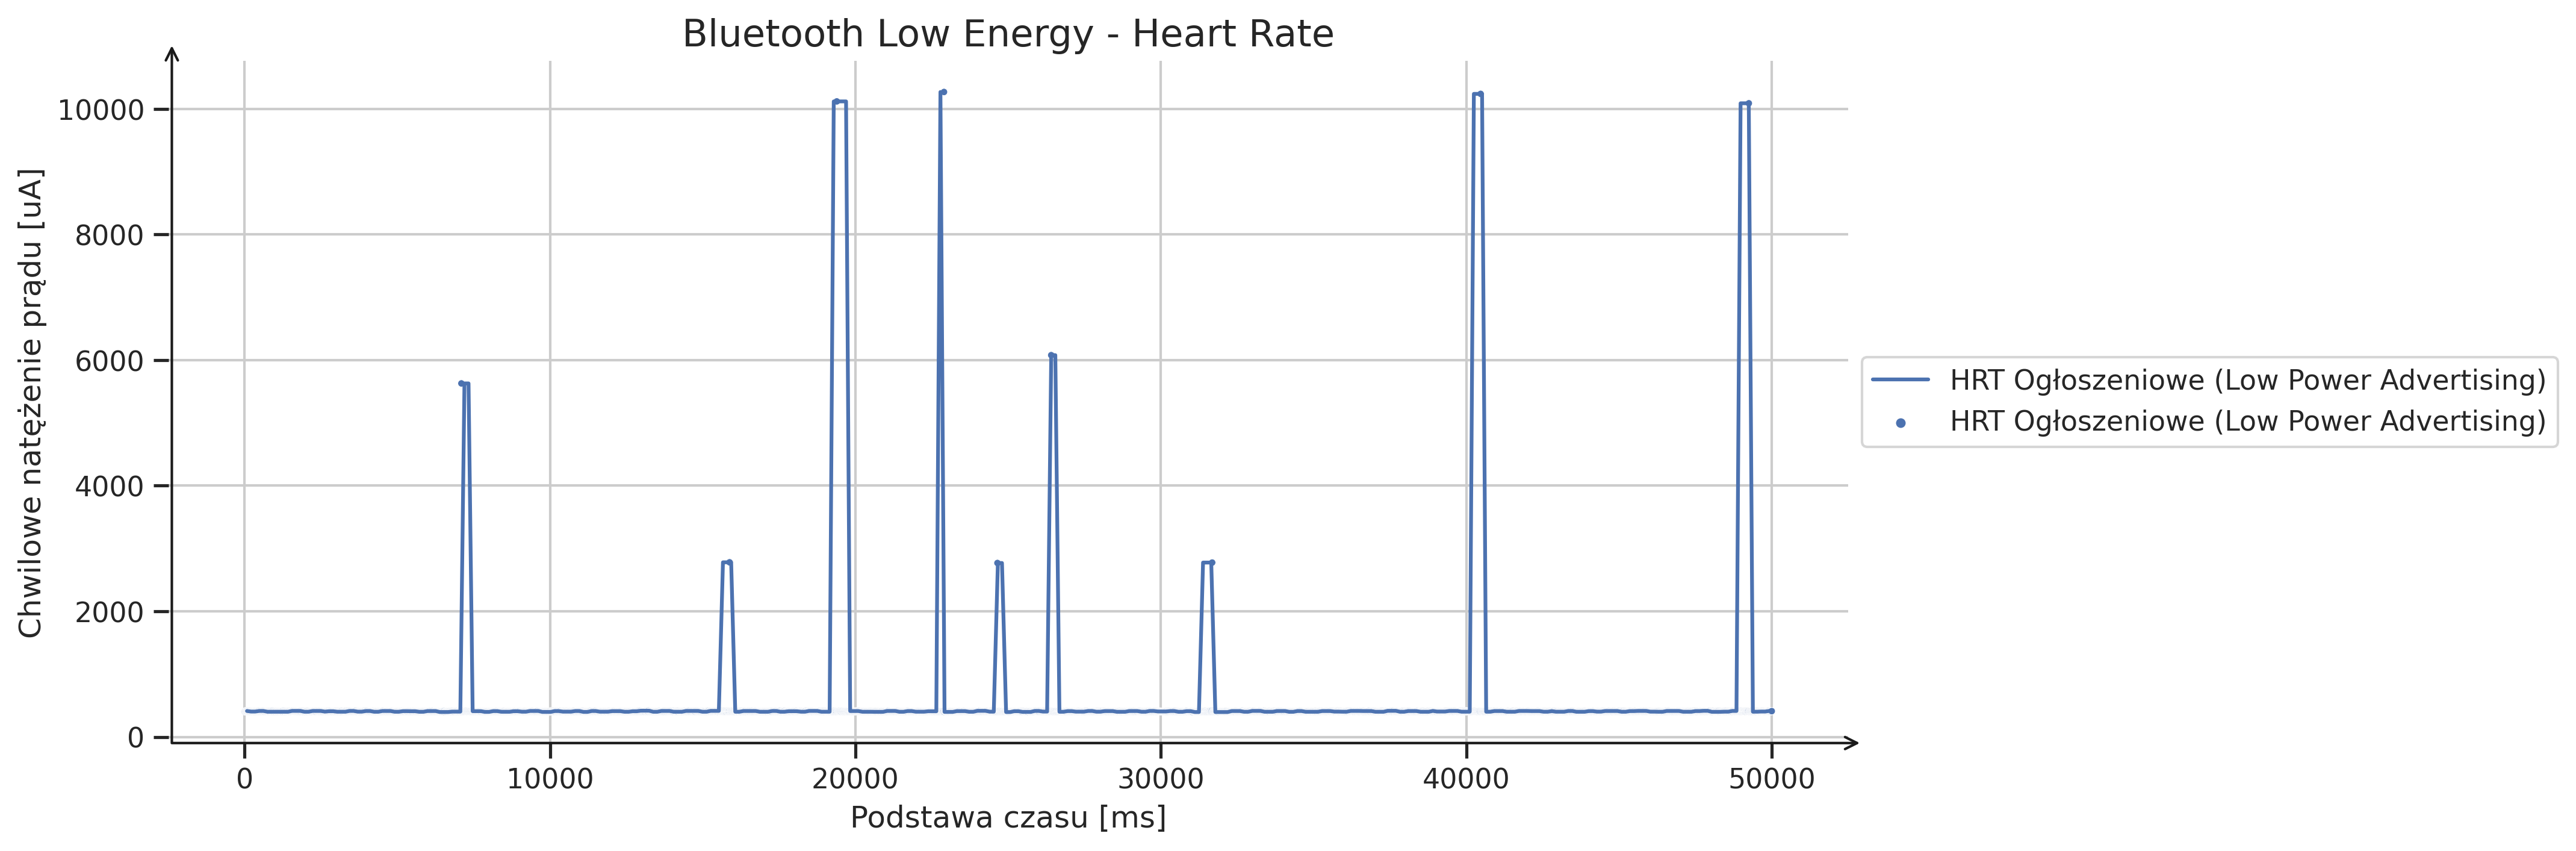
\includegraphics[width=0.99\linewidth]{power_ble_hr_low_power_adv_only_amps.png}
	\caption{Charakterystyka czasowa poboru prądu dla BLE i usługi Heart Rate - Tryb małomocowego ogłoszenia}
	\label{rys:power_ble_hr_low_power_adv_only_amps}
\end{figure}


\lipsum[1-2]
\begin{figure}[!htb]
	\centering 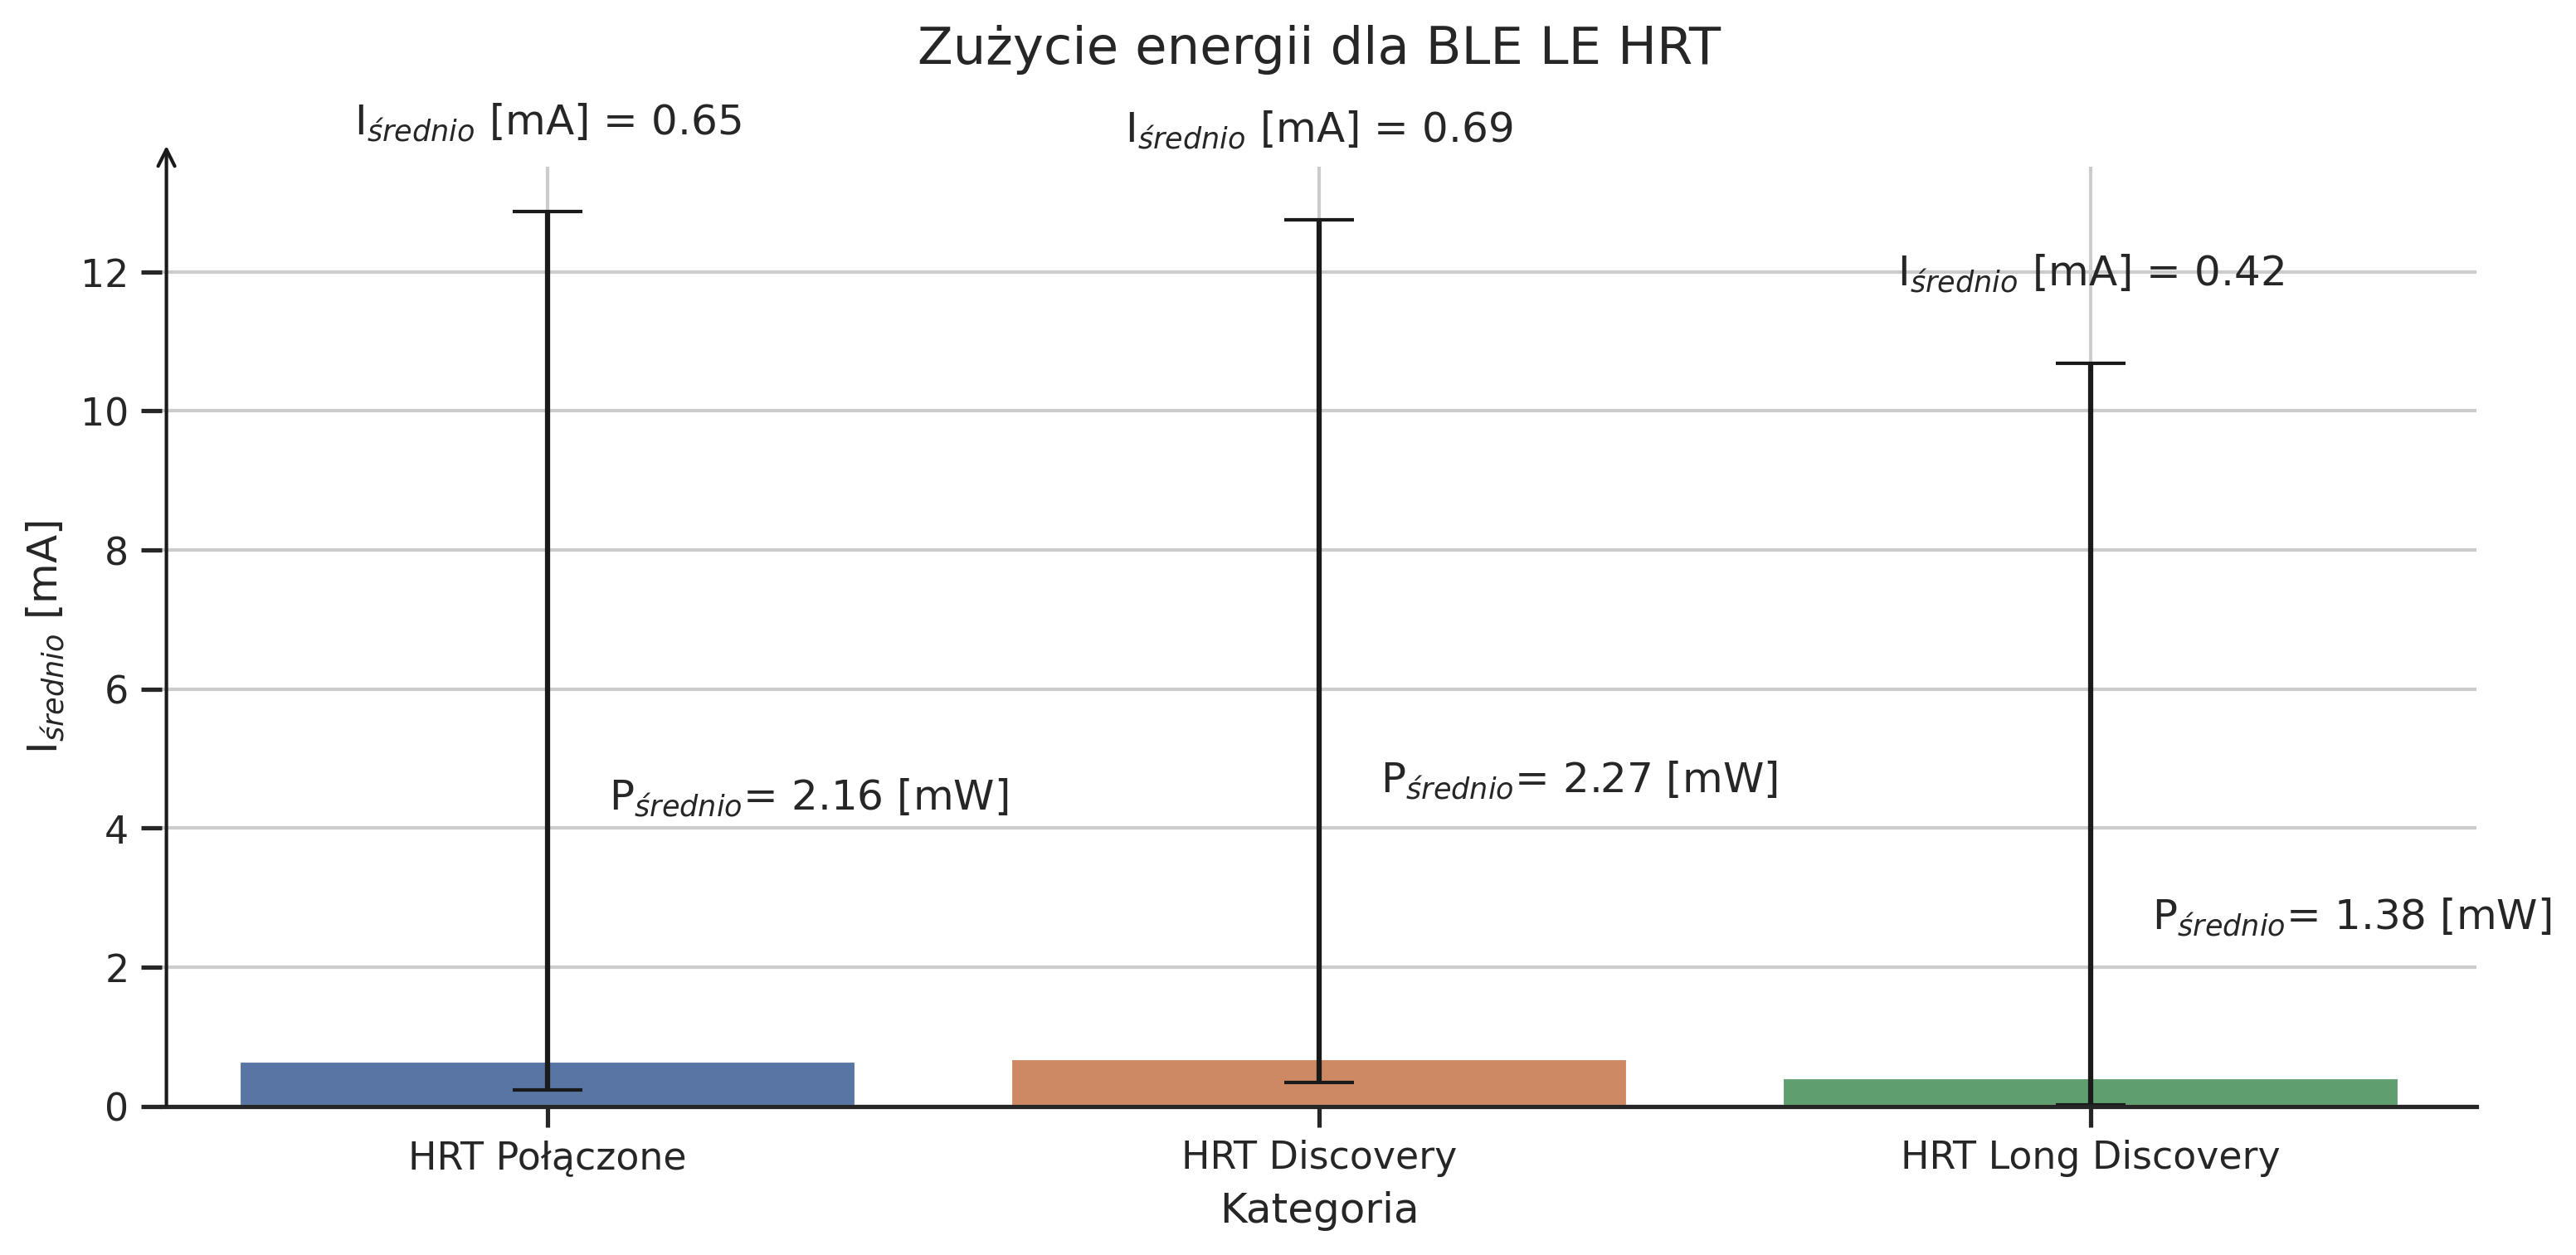
\includegraphics[width=0.99\linewidth]{power_ble_hr_amps_usage_juxtaposition.png}
	\caption{Zestawienie zużycia prądu dla usługi Heart Rate w zależności od trybu działania}
	\label{rys:power_ble_hr_amps_usage_juxtaposition}
\end{figure}
\lipsum[1-3]

%%%%%%%%%%%%%%%%%%%%%%%%%%%%%%%%%%%%%%%%%%%%%%%%%%%%%%%%%%%%%%%%%%%%%%%%%%%%%%%%
%% SUBSECTION: BLE Mesh - Model Generic OnOff
%%%%%%%%%%%%%%%%%%%%%%%%%%%%%%%%%%%%%%%%%%%%%%%%%%%%%%%%%%%%%%%%%%%%%%%%%%%%%%%%
\subsection{BLE Mesh - Model Generic OnOff}

Pomiary dla BLE Mesh uwzględniające dwa tryby działania: sieć w oczekująca na komunikaty oraz podczas działania aktywnego korzystania z Modelu Generic OnOff.

\begin{figure}[!htb]
	\centering 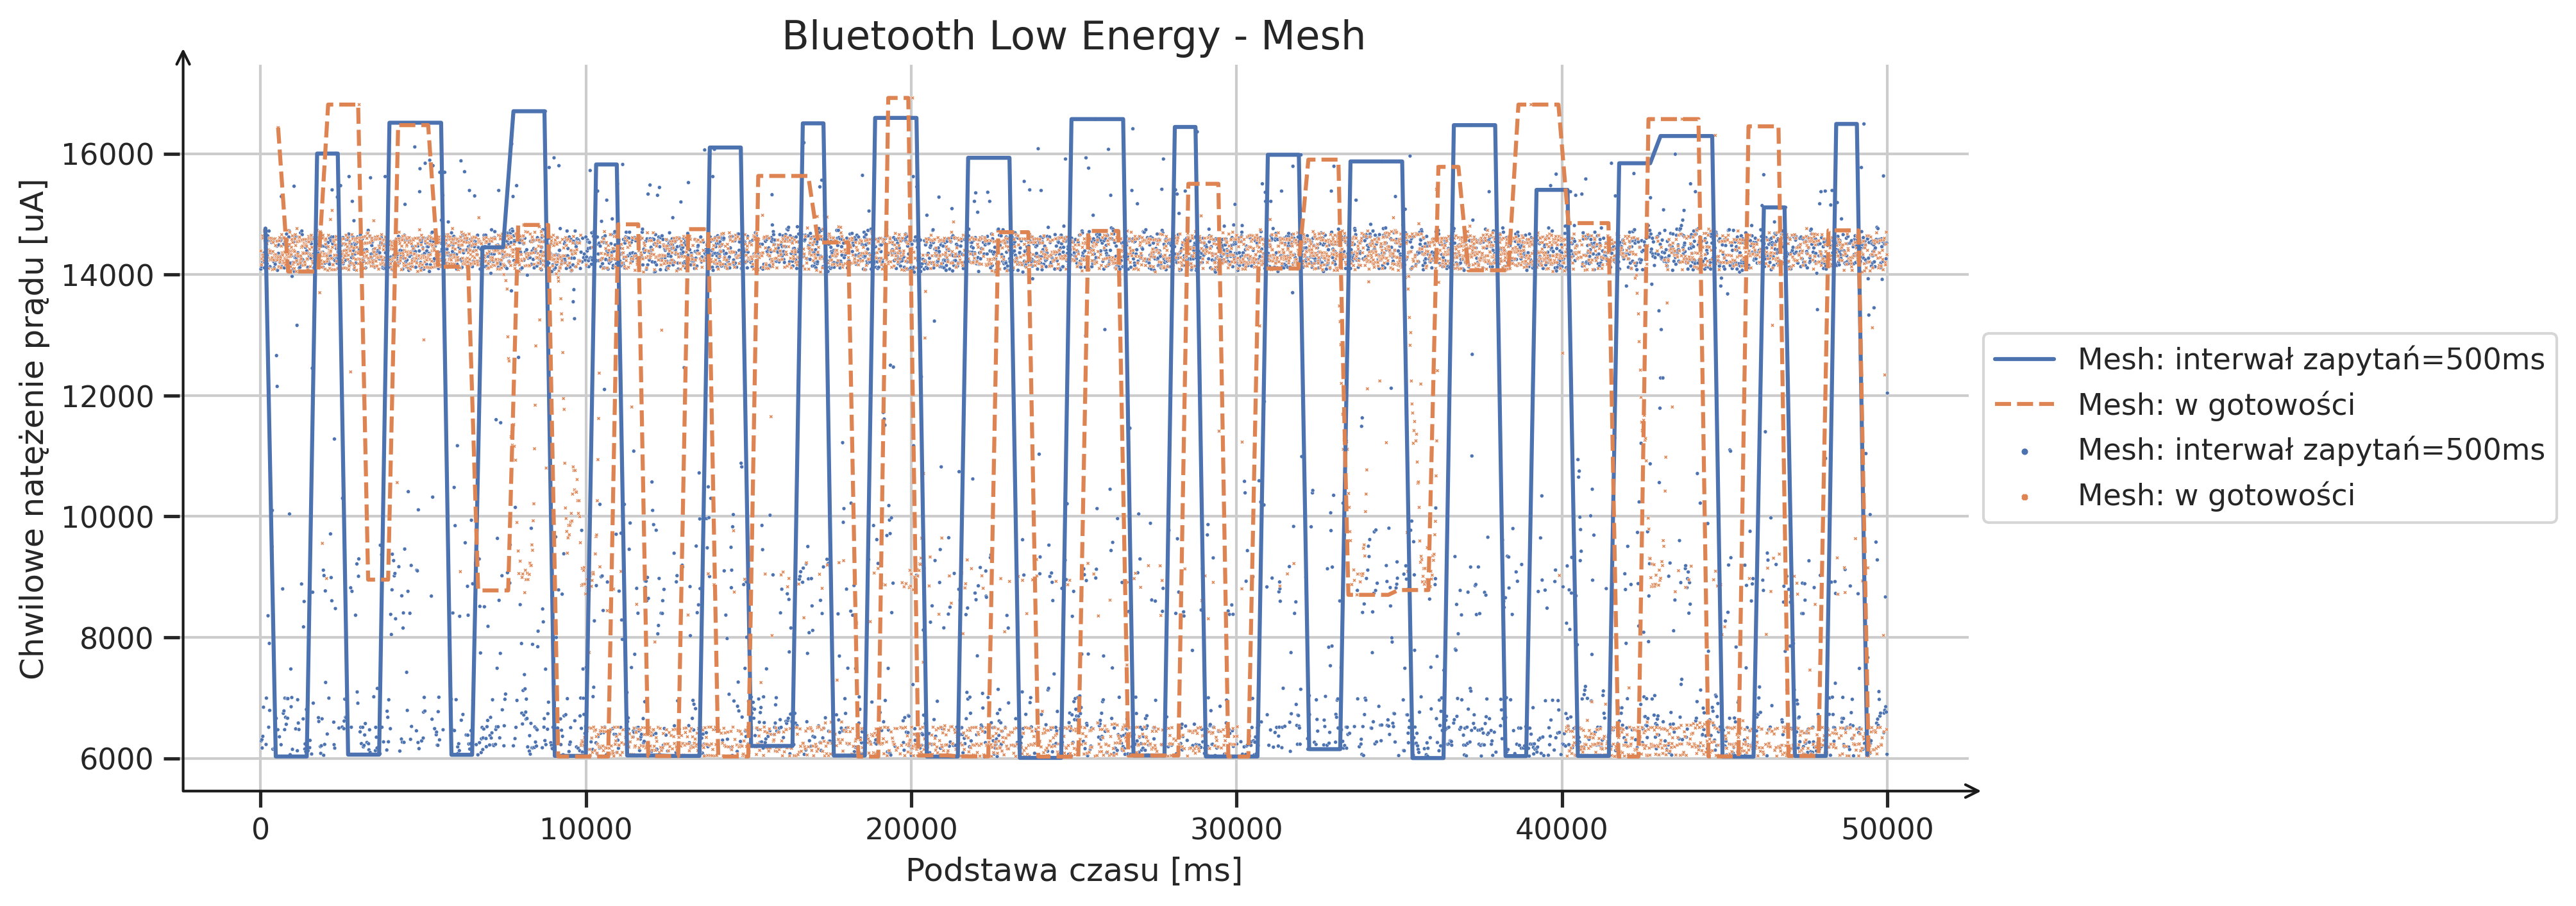
\includegraphics[width=0.99\linewidth]{power_ble_mesh_amps_no_led.png} 
	\caption{Charakterystyka czasowa poboru prądu dla BLE Mesh i modelu Generic OnOff}
	\label{rys:power_ble_mesh_amps}
\end{figure}

\lipsum[1-3]
\begin{figure}[!htb]
	\centering 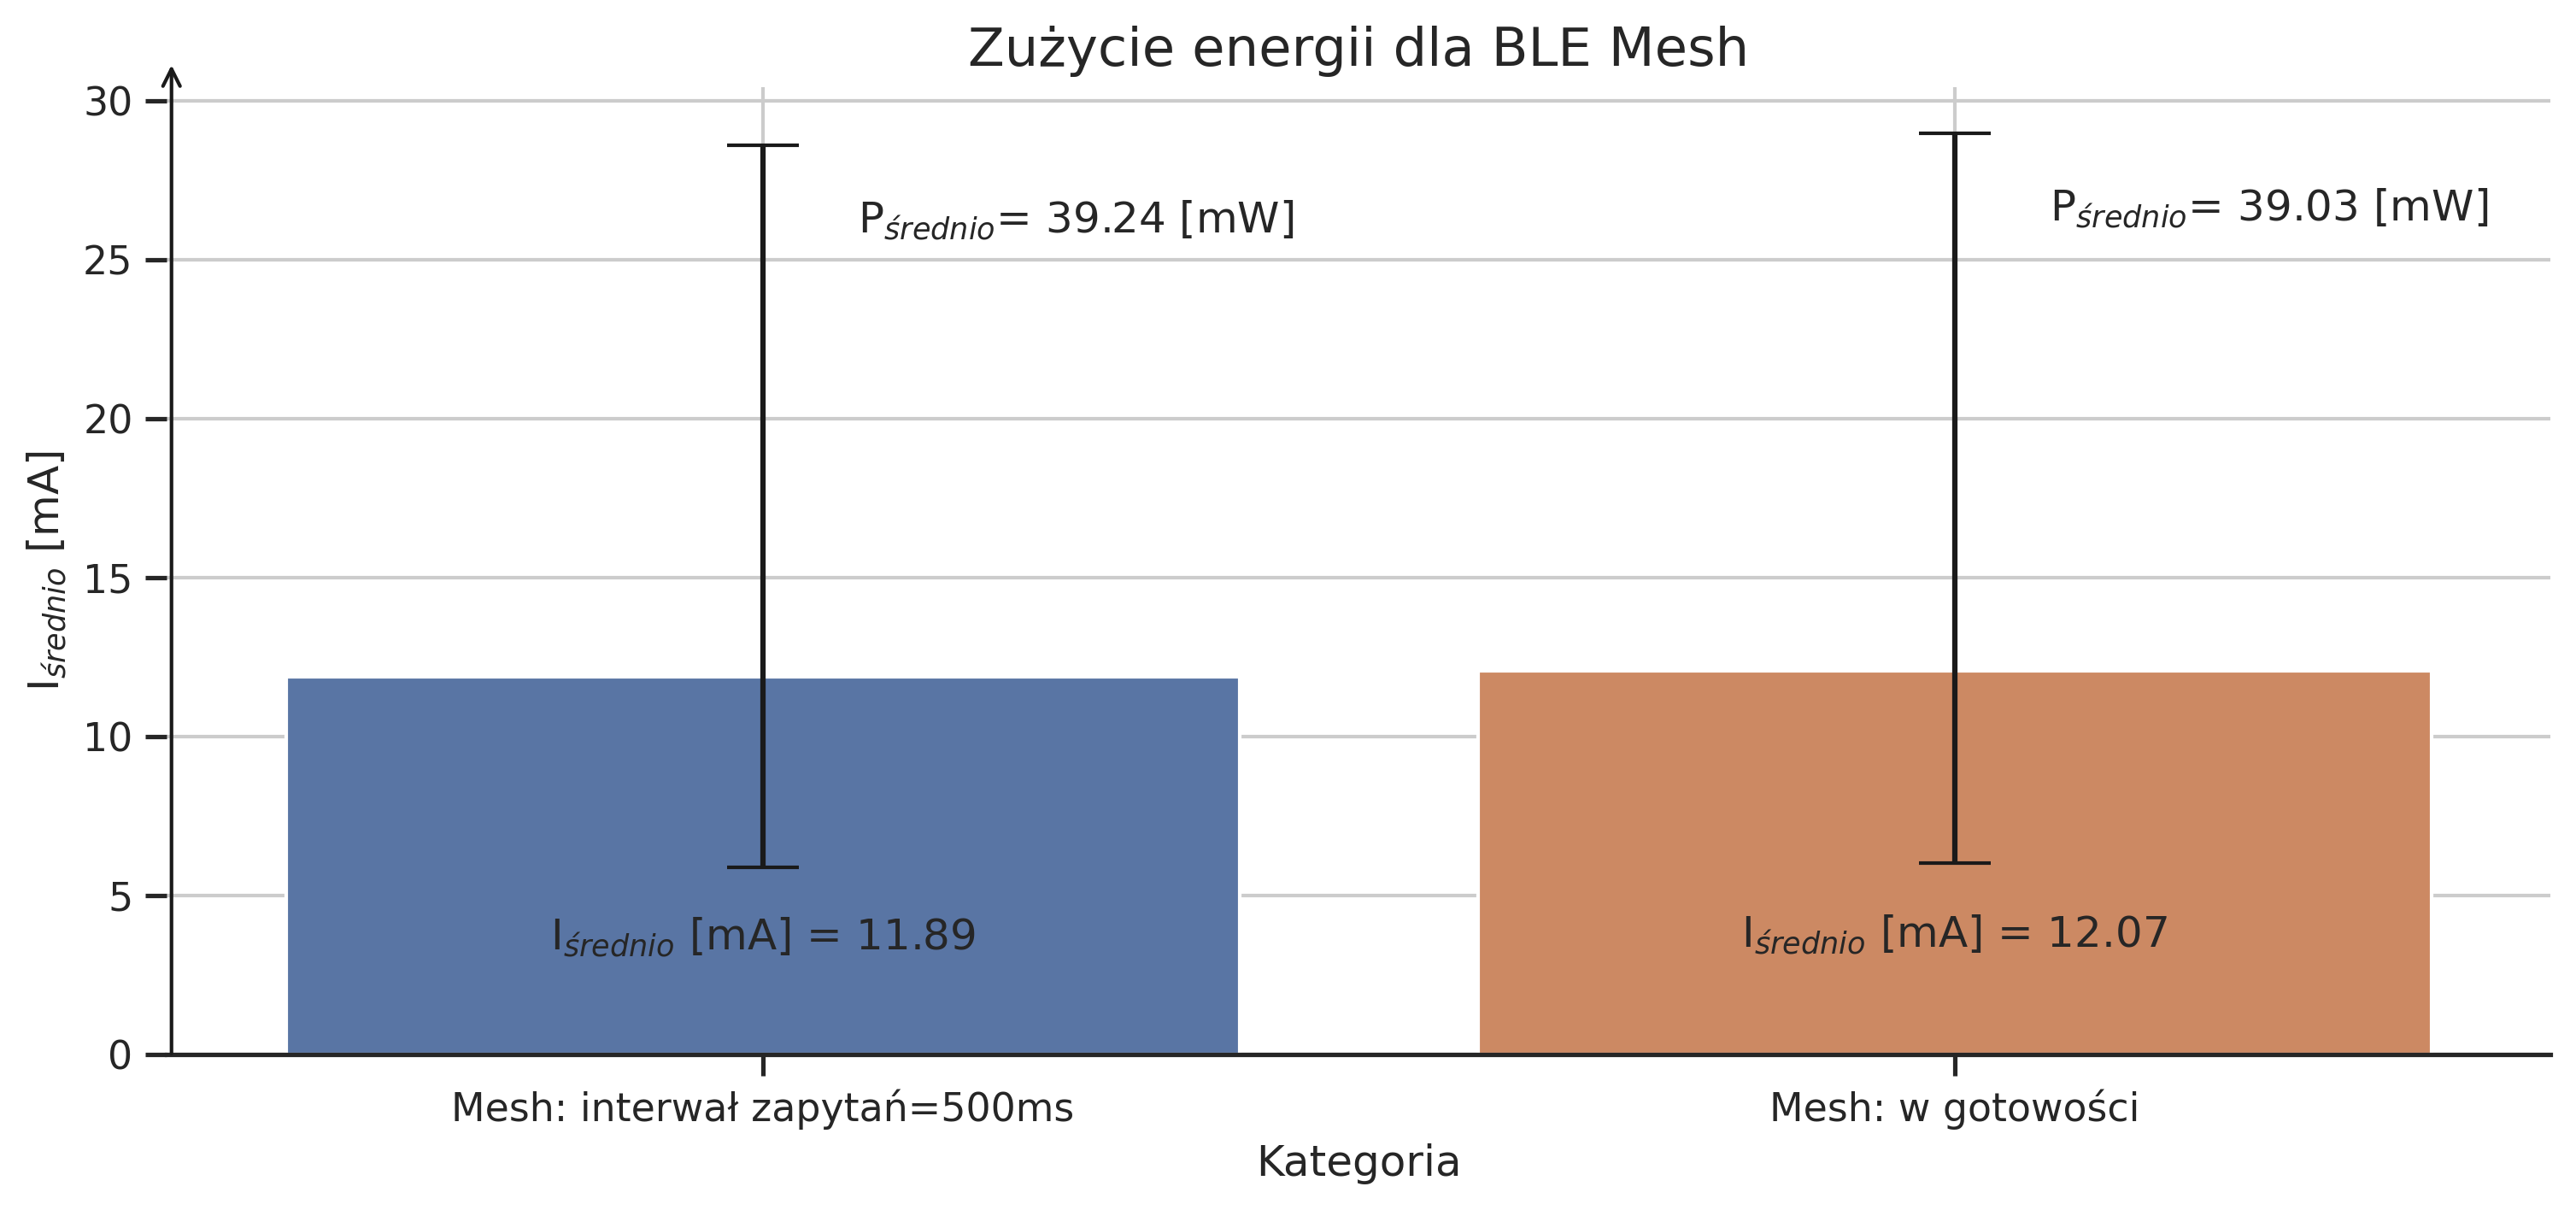
\includegraphics[width=0.99\linewidth]{power_ble_mesh_amps_usage_juxtaposition_no_led.png} 
	\caption{Zestawienie zużycia prądu dla BLE Mesh w zależności od trybu działania}
	\label{rys:power_ble_mesh_amps_usage_juxtaposition}
\end{figure}

\lipsum[1-3]
\begin{figure}[!htb]
	\centering 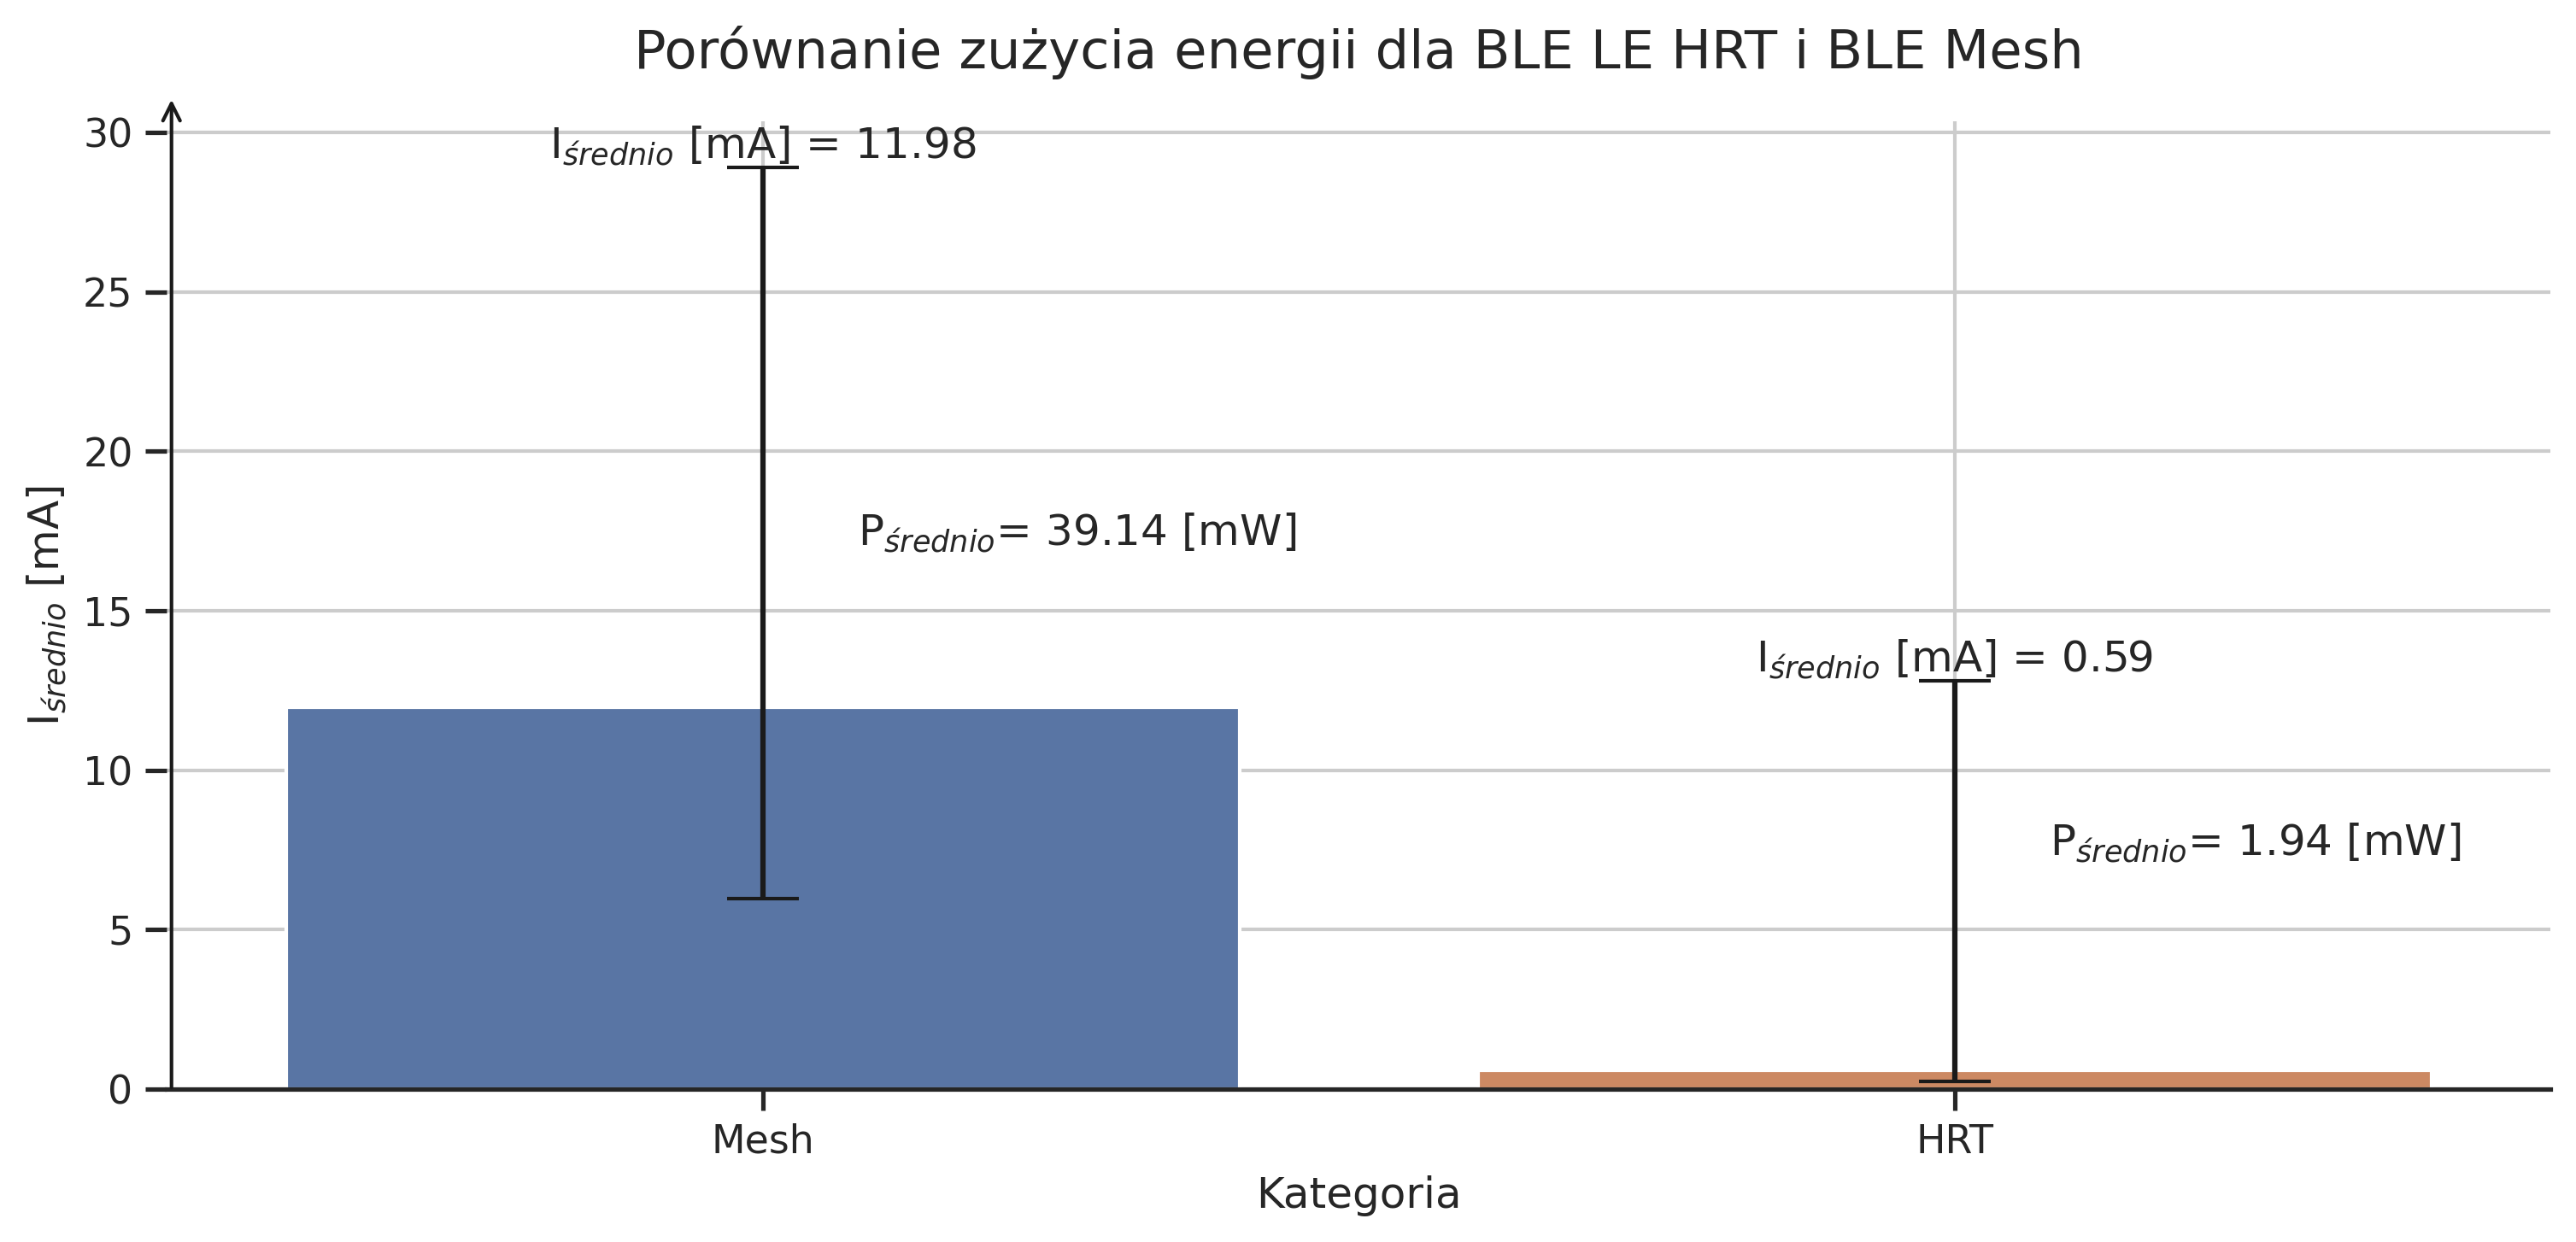
\includegraphics[width=0.99\linewidth]{power_ble_consumption_comparison_no_led.png} 
	\caption{Porównanie średniego zużycia energii pomiędzy BT Low Energy HRT i BLE Mesh}
	\label{rys:power_ble_consumption_comparison}
\end{figure}




%%!!!!!!!!!!!!!!!!!!!!!!!!!!!!!!!!!!!!!!!!!!!!!!!!!!!!!!!!!!!!!!!!!!!!!!!!!!!!!!
%%%%%%%%%%%%%%%%%%%%%%%%%%%%%%%%%%%%%%%%%%%%%%%%%%%%%%%%%%%%%%%%%%%%%%%%%%%%%%%%
%% SECTION: Packet Error Rate
%%%%%%%%%%%%%%%%%%%%%%%%%%%%%%%%%%%%%%%%%%%%%%%%%%%%%%%%%%%%%%%%%%%%%%%%%%%%%%%%
%%!!!!!!!!!!!!!!!!!!!!!!!!!!!!!!!!!!!!!!!!!!!!!!!!!!!!!!!!!!!!!!!!!!!!!!!!!!!!!!
\section{Packet Error Rate}

Celem niniejszego podrozdziału jest omówienie przeprowadzonego eksperymentu \gls{PER}. Omówiona zostanie
metodologia badań. Zdefiniowany zostanie termin \textit{pakietu}, który stanowi podstawę dla
doświadczenia.

Wychodząc z definicji, prezentuje się właściwy wzór matematyczny, definiujący badany problem. Równanie
stanowi podstawę dla eksperymentu. Jego zrozumienie pozwoliło zaprojektowanie właściwego doświadczenia
jak i~przygotowanie kompletnego stosu technologicznego niezbędnego do jego przeprowadzenia.

Ostatecznym efektem przeprowadzonego eksperymentu jest przedstawienie zebranych danych pod postacią
wykresów. Prezentują one badane cechy zmienne zaprezentowane w sekcji opisu metodologii. Końcowym
krokiem jest wyciągnięcie wniosków z zebranych danych.
 
\section{Packet Error Rate}

Celem niniejszego podrozdziału jest omówienie przeprowadzonego eksperymentu \gls{PER}. Omówiona zostanie
metodologia badań. Zdefiniowany zostanie termin \textit{pakietu}, który stanowi podstawę dla
doświadczenia.

Wychodząc z definicji, prezentuje się właściwy wzór matematyczny, definiujący badany problem. Równanie
stanowi podstawę dla eksperymentu. Jego zrozumienie pozwoliło zaprojektowanie właściwego doświadczenia
jak i~przygotowanie kompletnego stosu technologicznego niezbędnego do jego przeprowadzenia.

Ostatecznym efektem przeprowadzonego eksperymentu jest przedstawienie zebranych danych pod postacią
wykresów. Prezentują one badane cechy zmienne zaprezentowane w sekcji opisu metodologii. Końcowym
krokiem jest wyciągnięcie wniosków z zebranych danych.
 
%%%%%%%%%%%%%%%%%%%%%%%%%%%%%%%%%%%%%%%%%%%%%%%%%%%%%%%%%%%%%%%%%%%%%%%%%%%%%%%%
%% SUBSECTION: Zależność PER względem odległości między węzłami
%%%%%%%%%%%%%%%%%%%%%%%%%%%%%%%%%%%%%%%%%%%%%%%%%%%%%%%%%%%%%%%%%%%%%%%%%%%%%%%%
\subsection{Metodologia badania}
% poniższe sekcje przerzucić do części teoretycznej
\subsubsection{Definicja pakietu}
Przed przystąpieniem do badań należy precyzyjnie zdefiniować wykorzystywaną terminologię.

Pakietem nazywamy pojedynczą porcję danych przetwarzaną na poziomie warstwy sieciowej modelu ISO OSI \cite{sa_tcpip_nodate}.
Warstwa ta umożliwia routing, adresowanie logiczne oraz przetwarzanie i~dostarczanie pakietów.

\begin{figure}[!ht]
	\centering 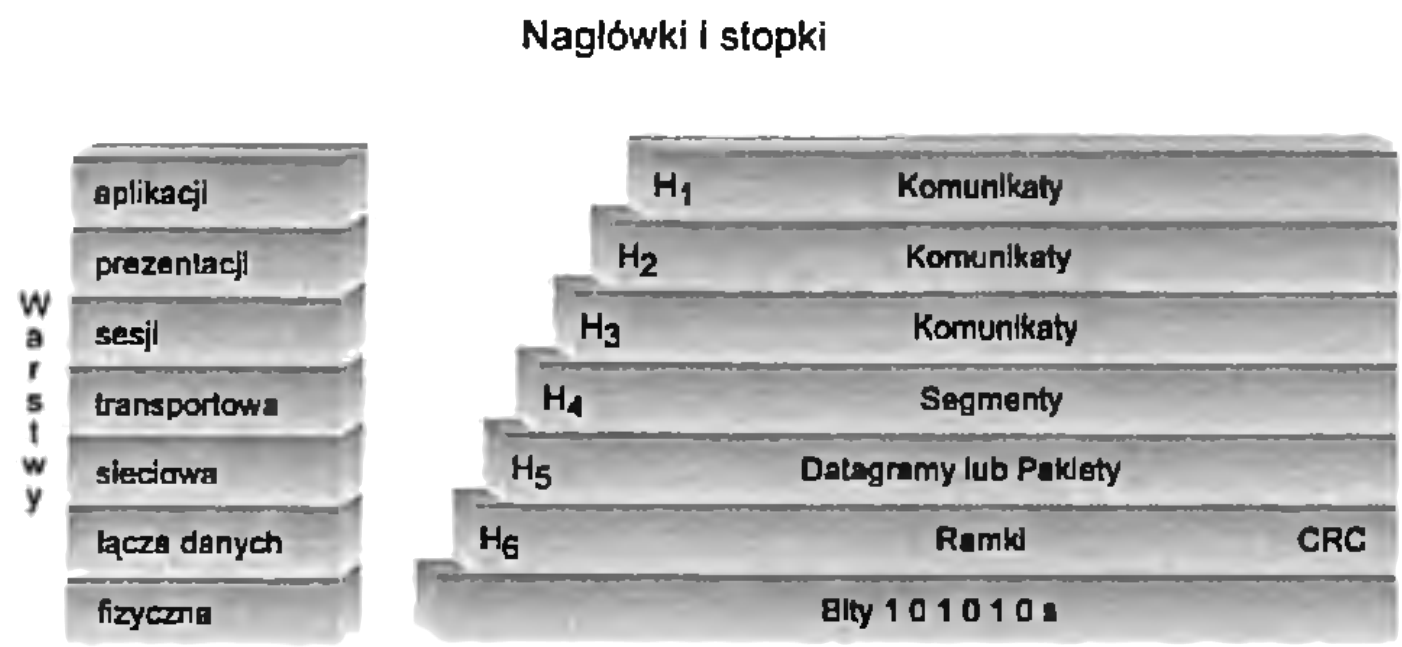
\includegraphics[width=0.618\linewidth]{tcp_ip_szkola_programowania_naglowki_stopki.png} 
	\caption{Model ISO OSI wraz i odpowiadające mu nazwy porcji danych. Źródło: \cite{sa_tcpip_nodate}}
	\label{rys:iso_osi_model_nazwy_grup_danych}
\end{figure}

\gls{BLE} wprowadza własną nomenklaturę dla poszczególnych warstw sieciowych. Jest to o tyle istotne, iż standard ten
nie zapewnia odpowiadających modelowi ISO OSI warstw jeden-do-jednego. Część z tych warstw jest agregowanych w~zespół 
protokołów wyższych warstw - Rysunek~\ref{rys:agregacja_protokolow_ble}. 

Bazując na definicji modelu OSI oraz stosie BLE, pakietem można nazwać wiadomości będące możliwie blisko
warstwy \textit{\gls{LL}}. Podobną definicję prezentuje dokumentacja ST:
\enquote{Pakiet to pojedyncza oznaczona wiadomość wysłana przez jedno i~odebrana przez 
co najmniej jedno urządzenie.}\footnote{Tłumaczenie własne}~\cite{stmicroelectronics_pm0271_2021}

\begin{figure}[!ht]
	\centering 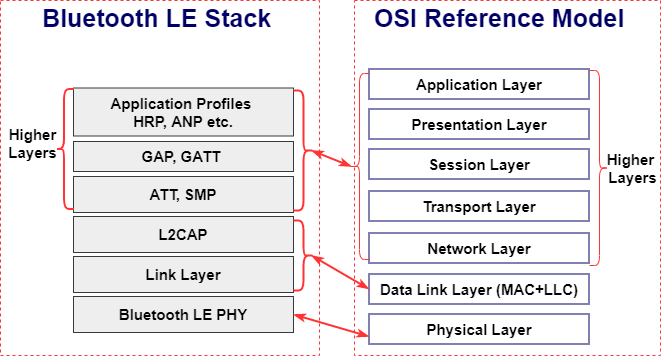
\includegraphics[width=0.618\linewidth]{mathworks_iso_osi_ble_stack.png} 
	\caption{Zestawienie stosu BLE i modelu ISO OSI. Źródło: \cite{noauthor_bluetooth_nodate}}
	\label{rys:agregacja_protokolow_ble}
\end{figure}

BLE Mesh dodatkowo wprowadza własne dodatkowe warstwy komunikacji, biorąc za podstawę stos BLE~\cite{mesh_working_group_mesh_2019}.
Każda z wymienionych warstw jest hermetyzowana za pośrednictwem dostarczanego przez producenta \gls{API}.
Uwzględniając zamknięcie middleware'u i dwu-procesorową architekturę mikrokontrolera STM32WB55, oznacza 
to brak możliwości bezpośredniego nasłuchiwania pakietów w~warstwie \gls{LL}.

Uwzględniając powyższe czynniki, \textit{pakietem} dla BLE Mesh nazywana będzie wiadomość najbliższa warstwie \gls{LL}.
W przypadku stworzonego oprogramowania, oznacza to odbiór komunikatu odebranego jako zdarzenie zarejestrowane przez
koprocesor Cortex-M0, będący integralną częścią mikrokontrolera STM32WB55 odpowiadający za obsługę radia.

\subsubsection{Definicja Packet Error Rate}
Posiadając definicję pakietu, \gls{PER} możliwe staje się zdefiniowanie wzoru, a zarazem znaczenia
głównego celu badań.

PER jest miarą ilości błędnych pakietów w proporcji do wszystkich wysłanych pakietów, zgodnie ze wzorem:

\begin{equation}
\label{per_equation}
PER = \frac{s - r}{s} \cdot 100\%
\end{equation}

gdzie:

\begin{description}
\item[s] is ilość wysłanych pakietów
\item[r] is ilość odebranych pakietów
\item[s-r] - ilość niepoprawnych/błędnych pakietów
\end{description}

Powyższy wzór stanowi podstawę eksperymentu pozwalającego wyznaczyć jakość łącza w zależności od
wybranych parametrów zmiennych.

\subsubsection{Procedura badawcza}\label{subsubsec:test-procedure}

Procedurę badawczą skonstruowano bazując na wzorze~\ref{per_equation}. Niezbędnym mechanizmem, o które oparte
jest doświadczenie, to zliczanie ilości pakietów. Zliczanie dotyczy zarówno węzła bliższego 
jak i~również węzła dalszego odbierającego wysyłane komunikaty. W przypadku drugiego elementu 
opracowano mechanizm odczytywania licznika zmian badanej wartości, patrz: \ref{prep:uc-software}.

Całość doświadczenia przeprowadzono z wykorzystaniem oprogramowania PC - \ref{prep:pc-software}. Oprogramowanie
zapewnia dwie główne funkcjonalności: wysyłanie komunikatów przy określonej częstości przez zadaną ilość czasu;
odczytywanie wartości licznika węzła dalszego.

Wysyłanym komunikatem jest polecenie zmiany stanu modelu
\textit{Generic OnOff}. Wybrano ten standardowy element stosu BLE Mesh ze względu na jego uniwersalność.
Nie ogranicza się on jedynie do wybranej platformy czy własnościowego modelu. Model ten jest zdefiniowany
przez Bluetooth SIG przez co jest niezależny od producenta. Czyni to eksperyment powtarzalny,
niezależnie od mikrokontrolera.

Odczytywanie stanu licznika wymagało wykorzystania autorskiego rozwiązania oparte o własnościowy model Mesh
ST. Nie wpływa to jednak na ostateczny rezultat badań, gdyż stworzone polecenia wykorzystywane jest
tylko do odczytu i~wysłania wartości licznika węzła dalszego do węzła bliższego i~komputera osobistego kontrolującego
przepływ doświadczenia. Z każdą kolejną próbą badania PER ten licznik jest automatycznie zerowany,
przez co sesja zliczeń zawsze rozpoczyna się od zera.

Eksperyment wyznaczający PER oparto o następujące czynniki zmienne:
\begin{itemize}
\item środowisko: teren leśny, teren zurbanizowany
\item interwał zapytań
\item dystans pomiędzy węzłami
\item ilość węzłów składających się na sieć Mesh
\end{itemize}


Wyznaczanie PER odbyło się w dwóch różnych środowiskach. Jednym z głównych hipotez jest znaczący wpływ
środowiska na jakość transmisji danych. Czynniki takie jak temperatura, wilgotność, rodzaj gleby czy
tło radiowe może mieć wpływ na komunikację pomiędzy węzłami. Założono, iż tło radiowe może mieć
największy wpływ ja transmisję danych. Stąd dobrano możliwie skrajne miejsca do badań oceniając
to jako najistotniejszy czynnik:
\begin{itemize}
\item Kampinowski Park Narodowy (lokalizacja: parking Roztoka) - jako teren leśny oddalony od ośrodka miejskiego
ze względnie niewielkim tłem radiowym. Pogoda: pochmurnie, wilgotno, temperatura poniżej 20$^{\circ}$C.
\item Park Pola Mokotowskie - jako teren zurbanizowany charakteryzujący się bogatym tłem radiowym działającym
w pasmach \gls{ISM}. Pogoda: słonecznie, temperatura ok. 20$^{\circ}$C.
\end{itemize}

Kolejnym badanym czynnikiem jest interwał zapytań. Parametr ten został wybrany ze względu na obserwowane
problemy z komunikacją podczas etapu tworzenia oprogramowania. Parametry dobrano w takim stopniu, by ów problem
ukazać. Obrano następujące interwały:
\begin{itemize} \label {items:ping_intervals}
\item 100ms
\item 500ms
\item 800ms
\item 1300ms
\item 2100ms
\end{itemize}

Interesującym parametrem dla bezprzewodowej transmisji danych jest zasięg. Stąd też, jednym z badanych czynników jest
określenie jakości PER w zależności od odległości - Rysunek~\ref{rys:two_nodes_setup}.
\begin{itemize}
\item 1,5m
\item 3,0m
\item 5,0m
\item 8,0m
\item 13,0m
\item 16,0m
\item 21,0m
\end{itemize}

\begin{figure}[!ht]
	\centering 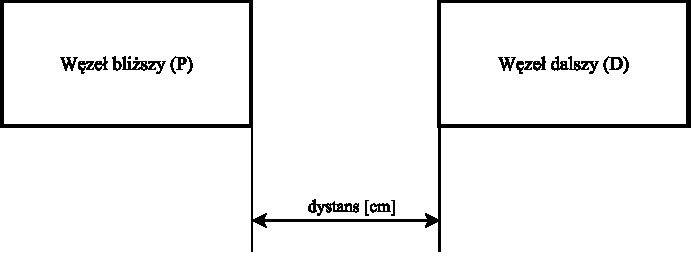
\includegraphics[width=0.618\linewidth]{per_two_nodes.pdf} 
	\caption{Dystans pomiędzy węzłami dla sieci dwóch mikrokontrolerów}
	\label{rys:two_nodes_setup}
\end{figure}

Wyżej wymienione odległości stosowano również w przypadku kolejnego badanego parametru, tj. ilości węzłów
składających się na sieć BLE. W celu łatwej identyfikacji węzłów, wprowadza się następujące nazewnictwo:
\begin{itemize}
	\item węzeł bliższy (ang./łac. \textit{proximal node}/\textit{nodus proximalis}) - węzeł będący połączony bezpośrednio
	ze stacją akwizycji danych i kontroli przepływu eksperymentu.
	\item węzeł środkowy (ang./łac. \textit{intermedial node}/\textit{nodus [inter]medius}) - węzeł działający w trybie
	przekaźnika (terminologia Mesh: \textit{Relay}). Węzeł ten nie uczestniczy bezpośrednio w badaniach tj. nie są
	z niego odczytywane jakiekolwiek dane.
	\item węzeł dalszy (ang./łac. \textit{distal node}/\textit{nodus distalis}) - węzeł zliczający ilość odebranych danych \textit{r},
	udostępniający jednocześnie usługę umożliwiającą odczyt tych wartości tak jak opisano to w podrozdziale \ref{prep:uc-software}.
\end{itemize}

Postanowiono o równoodległym rozstawieniu węzłów - Rysunek~\ref{rys:three_nodes_setup}. Dla sieci 3 węzłów,
maksymalna odległość dzieląca węzeł bliższy od węzła dalszego to 42m. Protokół badawczy zawiera informację 
tylko o odległości w~rozumieniu równoodległego rozstawienia węzłów. Odległość pomiędzy elementami 
jest oczywistą operacją arytmetyczną.

\begin{figure}[!ht]
	\centering 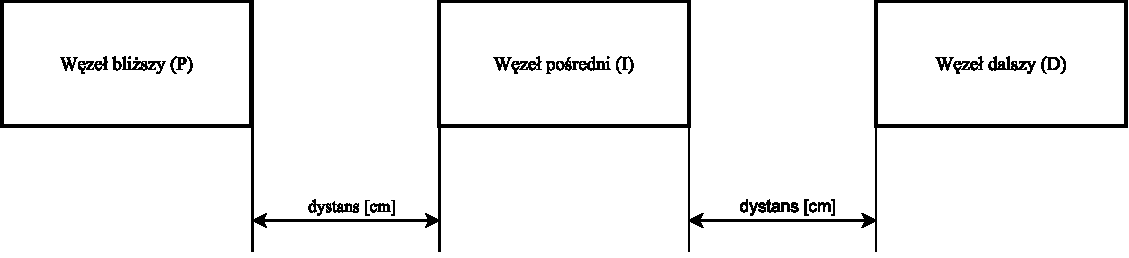
\includegraphics[width=0.99\linewidth]{per_three_nodes.pdf} 
	\caption{Dystans pomiędzy węzłami dla sieci trzech mikrokontrolerów}
	\label{rys:three_nodes_setup}
\end{figure}

Odległość pomiędzy węzłami mierzona jest z użyciem taśmy mierniczej z podziałką 1mm. Tolerancję pomiarów należy
przyjąć jako najdłuższy wymiar zestawu uruchomieniowego P-NUCLEO-WB55 - 70mm \cite{stmicroelectronics_um2435_2019}.
Pomiar odbywał się na płasko, mierząc odległość pomiędzy leżącymi na glebie węzłami. Błędy pomiarowe wynikłe
z ukształtowania terenu są prawdopodobne i~wynikają z~terenowego charakteru badań.

W celu zminimalizowania ryzyka pojawienia się losowych błędów o nieznanym pochodzeniu badanie powtarzano pięciokrotnie,
w sposób następujący: dla wybranego środowiska, ilości węzłów i zadanej odległości pomiędzy węzłami, wykonaj
5 powtórzeń pomiarowych dla każdego z zadanych interwałów pomiarowych.

\begin{equation}
\label{experiment_definition}
\exists e, \exists n, \exists d: PER_i = f(e, n, d), i=1,...,5
\end{equation}

gdzie:

\begin{description}
\item[e] - środowisko
\item[n] - ilość węzłów
\item[d] - równoodległy dystans pomiędzy węzłami
\item[i] - ilość powtórzeń
\item[PER] - Packet Error Rate dla wybranego powtórzenia przy stałych parametrach e, n, d
\end{description}

Wykorzystując tak zebrane dane, wyrysowano je na szeregu wykresów wyznaczając jednocześnie
linie aproksymacyjne z użyciem modelu liniowego wyznaczonego metodą najmniejszych kwadratów. Odchylenia standardowe zaprezentowane
są z użyciem ograniczonego tła otaczającego linię w tym samym kolorze o~zmienionym parametrze nieprzezroczystości.

Parametry transmisji danych nie ulegały zmianie podczas przeprowadzanych doświadczeń. Poniższe wartości należy
przyjąć za stałe:
\begin{itemize}
\item Szybkość transmisji: 2Mbps
\item Moc transmisji danych: 0dBm
\end{itemize}

%%%%%%%%%%%%%%%%%%%%%%%%%%%%%%%%%%%%%%%%%%%%%%%%%%%%%%%%%%%%%%%%%%%%%%%%%%%%%%%%
%% SUBSECTION: Zależność \gls{PER} względem częstości zapytań
%%%%%%%%%%%%%%%%%%%%%%%%%%%%%%%%%%%%%%%%%%%%%%%%%%%%%%%%%%%%%%%%%%%%%%%%%%%%%%%%
\subsection{Zależność PER względem częstości zapytań}

Pierwszą sprawdzaną hipotezą jest empiryczna weryfikacja czy częstość zapytań wpływa na \gls{PER}.
W tym celu wykreślono szereg wykresów dla wybranych interwałów czasowych. Pozostałe parametry traktowane są
jako stałe.

Rysunek~\ref{rys:per_to_distance_under_100ms} przedstawia zależność PER dla interwału 100 milisekund w~zależności
od odległości dla sieci złożonej z dwóch i trzech węzłów. 

\begin{figure}[!htb]
	\centering 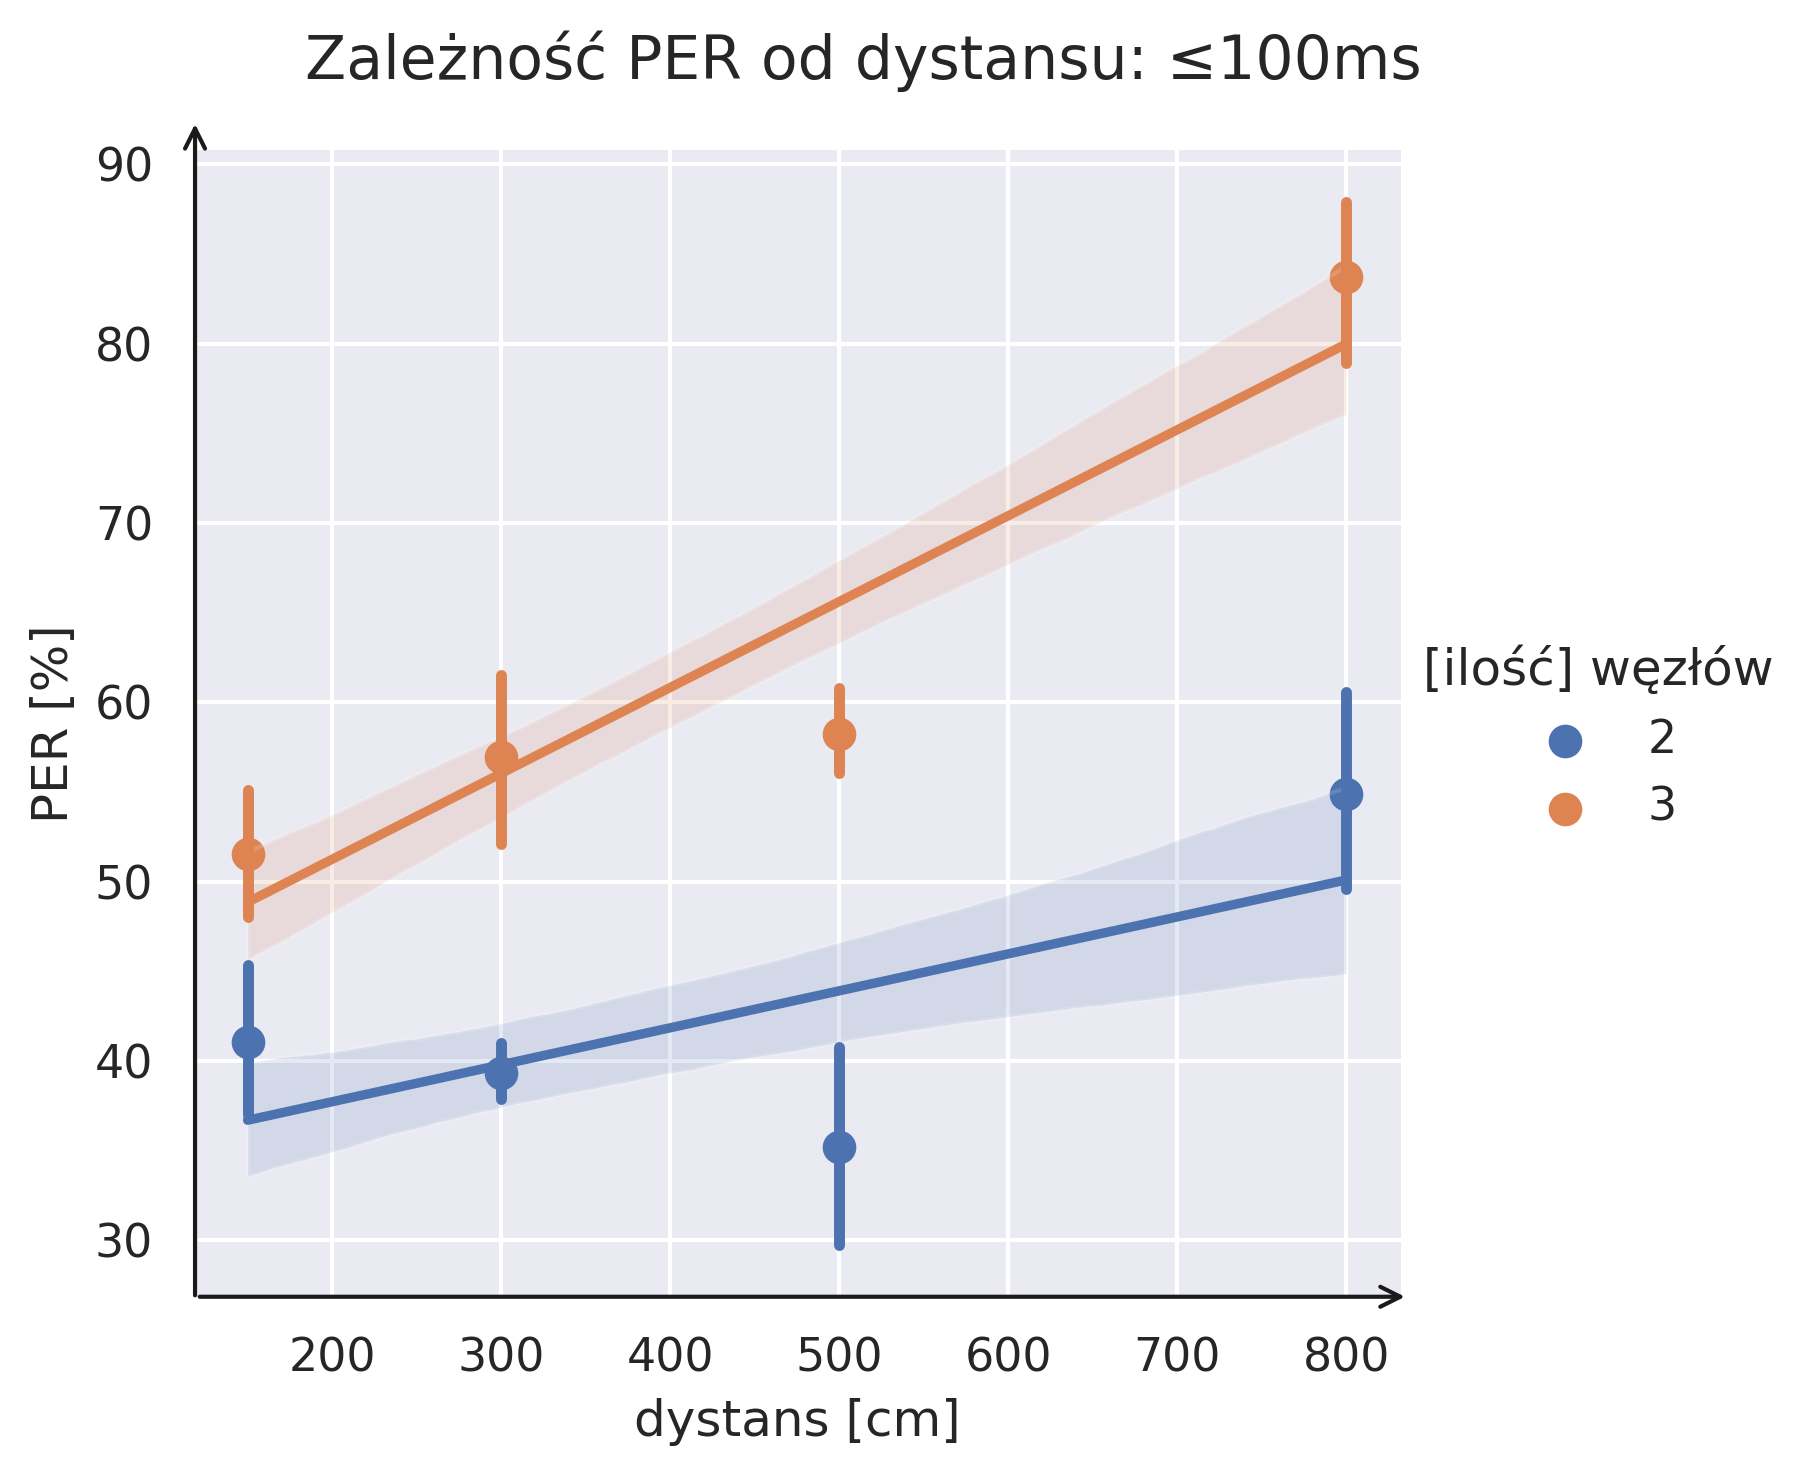
\includegraphics[width=0.618\linewidth]{per_to_distance_under_100ms.png}
	\caption{Zależność \gls{PER} od dystansu dla zapytań o częstości $\leqslant$ 100ms dla różnej liczby węzłów}
	\label{rys:per_to_distance_under_100ms}
\end{figure}

Niewątpliwą cechą ukazanych danych jest wysoka wartość PER już przy tak niewielkiej odległości jak 150 cm pomiędzy węzłami.
Utrata 40-50\% wysyłanych pakietów danych już na pierwszym dystansie pomiarowym może być spowodowana wieloma czynnikami.
Przypuszczalnie, wpływ na taki rezultat wywodzi się z czynników środowiskowych lub ze sposobu wykonywania 
eksperymentu. Niewykluczone są również ograniczenia sprzętowe.

Wraz ze wzrostem odległości pomiędzy węzłami PER wzrasta pomimo wysokiej wartości początkowej. Jest to 
oczekiwana zależność i zgodna z wiedzą techniczną.

Prowadząc dalszą analizę zależności PER od częstości zapytań, sprawdzono wpływ środowiska na jakość transmisji danych.
Rysunek~\ref{rys:per_to_distance_under_100ms_different_envs} przedstawia wybraną zależność. Rozróżnienie
na ilość węzłów nie zostało tutaj uwzględnione. Pomiary przeprowadzone w~najbliższym dobranym dystansie ponownie 
wskazują na 40-50\% utratę pakietów w węźle dalszym. Analogiczne rezultaty obserwowane są na pozostałych dystansach 
z~oczekiwaną tendencją wzrostową.
Wykres dodatkowo przedstawia pewną różnicę w jakości transmisji danych w~zależności od środowiska. Różnica ta 
jednak mieści się w odchyleniu standardowym, posiadając część wspólną dla zadanych parametrów. Nie jest to 
wystarczające do stwierdzenia jednoznacznego wpływu środowiska.

\begin{figure}[!htb]
	\centering 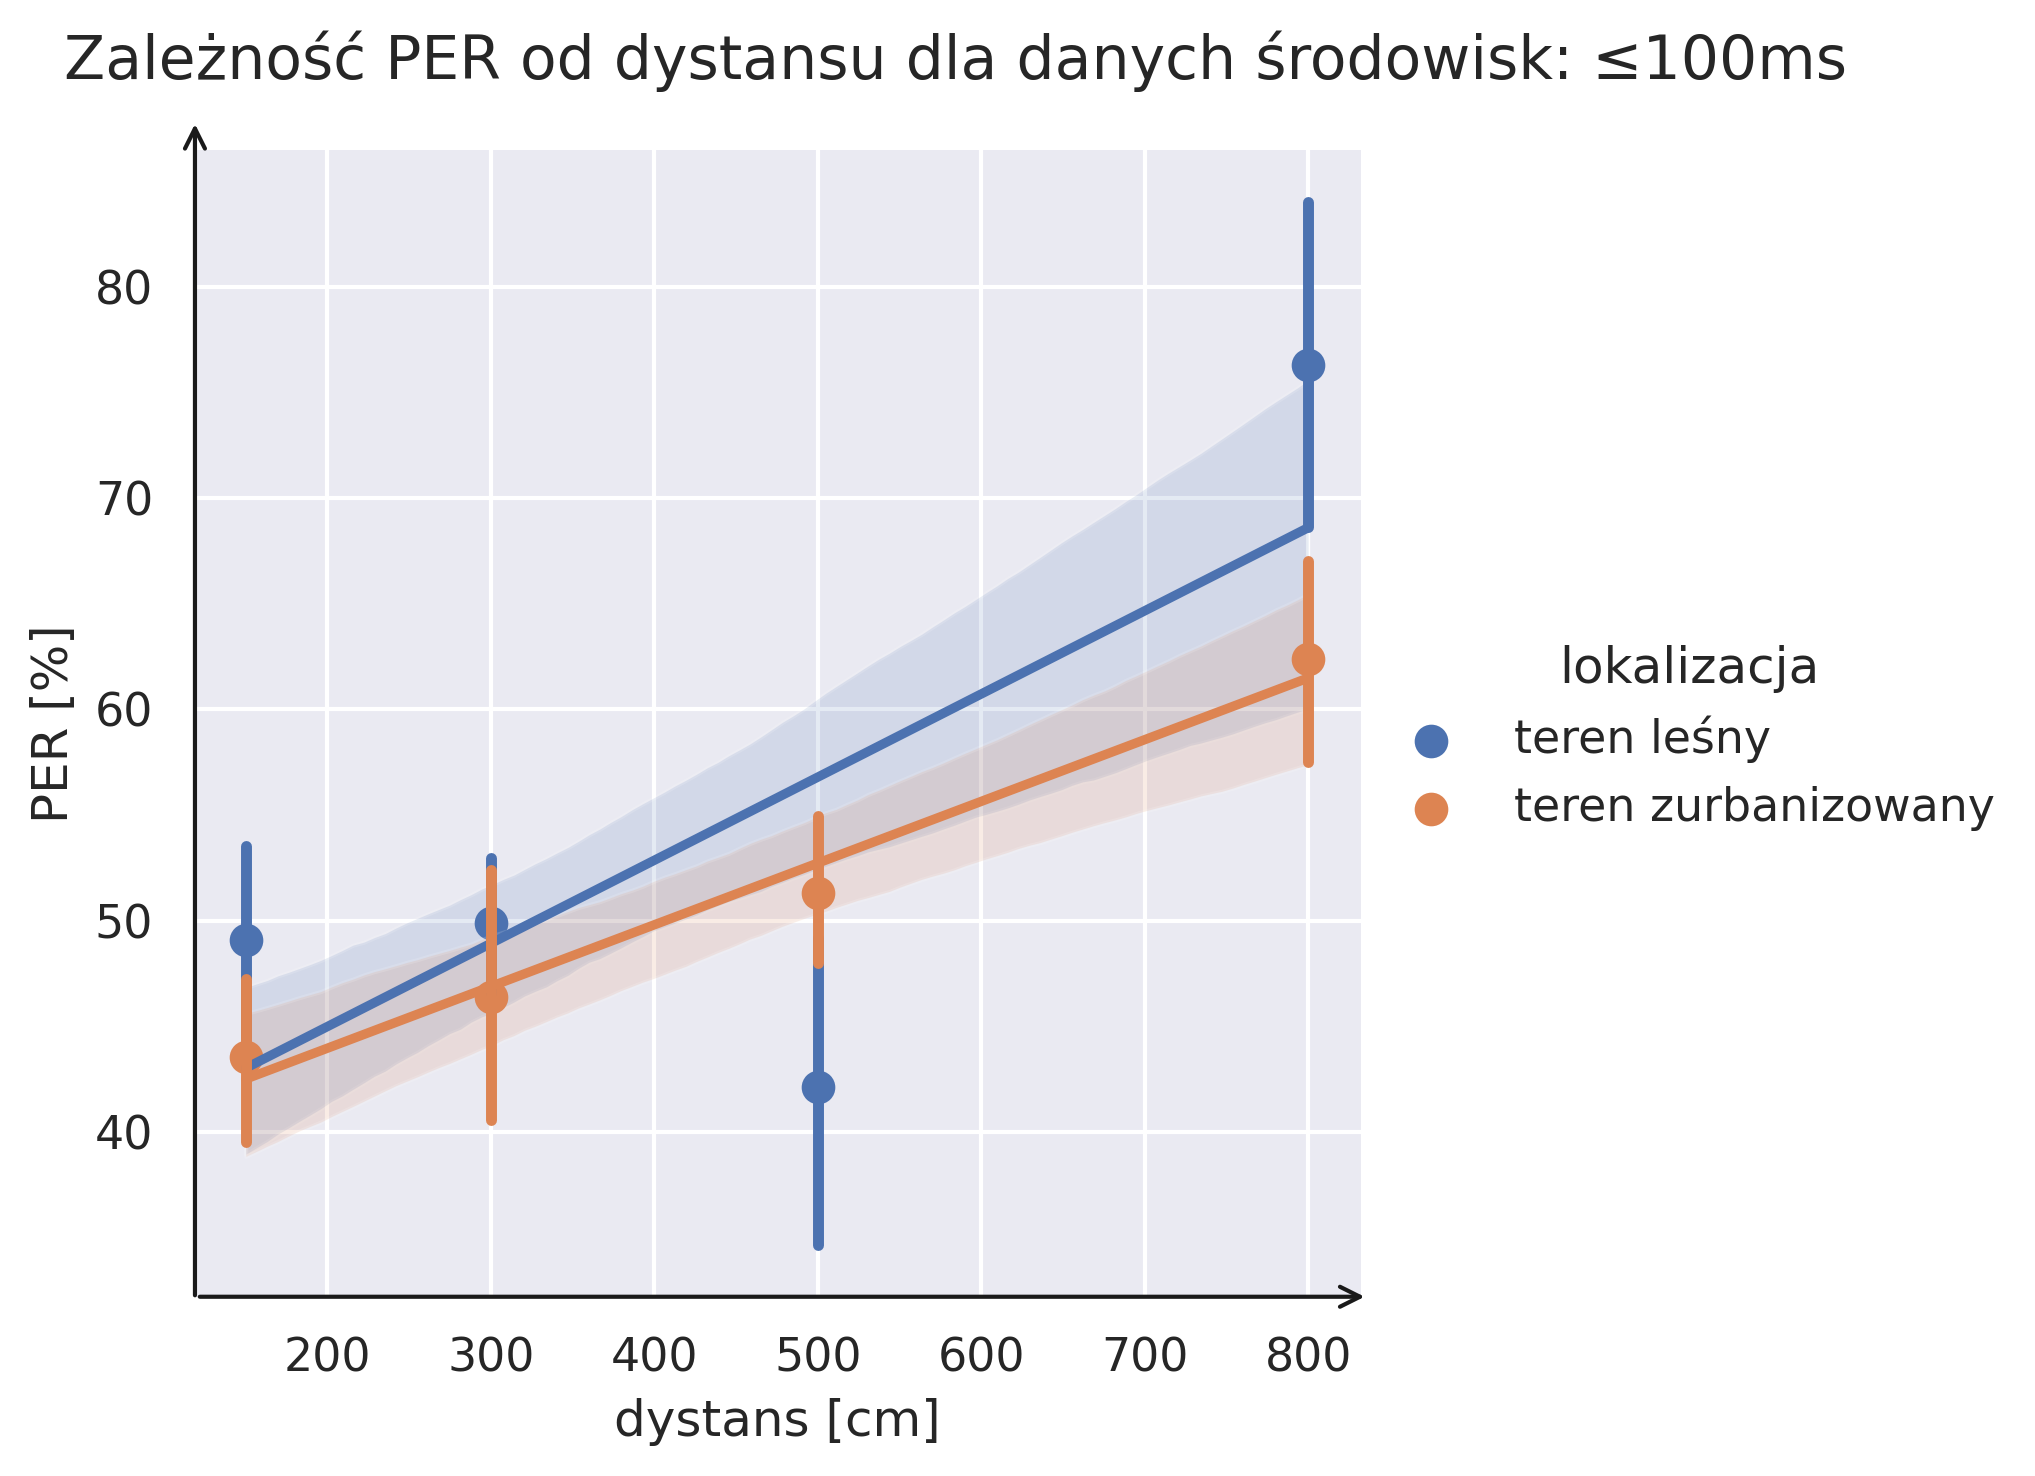
\includegraphics[width=0.618\linewidth]{per_to_distance_under_100ms_different_envs.png} 
	\caption{Zależność \gls{PER} od dystansu dla zapytań o częstości $\leqslant$ 100ms w wybranych środowiskach bez rozróżnienia na liczbę węzłów}
	\label{rys:per_to_distance_under_100ms_different_envs}
\end{figure}

Zestawiając ze sobą wymienione wcześniej czynniki, obserwuje się interesujące zależności. Rysunek~\ref{rys:per_to_distance_under_100ms_different_envs_and_nodes} wskazuje na zależność dystansu, ilości węzłów i rodzaju
środowiska dla wybranego interwału zapytań 100 milisekund. Po raz kolejny obserwowany jest PER wynoszący
40-50\%, niezależnie od środowiska czy ilości węzłów. Sugeruje to wpływ samej testowanej platformy
na ostateczny rezultat. Prawdopodobną hipotezą jest niewystarczająca wielkość zaalokowanych
buforów obsługujących transmisję danych. Mikrokontroler nie będąc w stanie obsłużyć tak częstej transmisji
może doświadczyć awarii, co zaobserwowano podczas badań. Awaria objawiała się brakiem reakcji węzła bliższego
na jakiekolwiek komendy AT, co wymagało ponownego uruchomienia urządzenia. Weryfikacja tego zagadnienia
wymagałaby zaangażowania zaawansowanych narzędzi programistycznych ingerujących m.in. w~pamięć urządzenia.
Niniejsza praca nie podejmuje się wyjaśnienia przyczyn obserwowanych anomalii w działaniu mikrokontrolera,
udostępniając jednocześnie możliwy punkt dla dalszych prac badawczych z zakresu BLE Mesh.

Wpływ samego stosu łączności na PER przy zadanej częstości zapytań zdaje się potwierdzać wykres uwzględniający
jakość transmisji dla dwóch węzłów. Niemalże pozioma linia aproksymacji sugeruje niewielki wpływ dystansu na PER.
Dotyczy to zarówno terenu zurbanizowanego jak i~terenu leśnego. Zbliżone rezultaty zdają się wykluczać
czynniki zewnętrzne.

Interesującą zależnością jest nachylenie wykresu względem osi odciętych. Dla przypadku dwóch węzłów sieci,
połączenie bezpośrednio między węzłami, PER jest niemal stałe na wybranych odległościach, porównywalne
z~przypadkiem terenu leśnego. W przypadku trzech
węzłów, uwidacznia się potencjalny wpływ węzła środkowego, przekazującego pakiety z punktu bliższego do
dalszego. Wraz ze wzrostem dystansu, rośnie wartość PER sięgając nawet 90\% w terenie leśnym. Różne nachylenie
dla wybranych środowisk również sugeruje znaczący wpływ środowiska na PER.

\begin{figure}[!htb]
	\centering 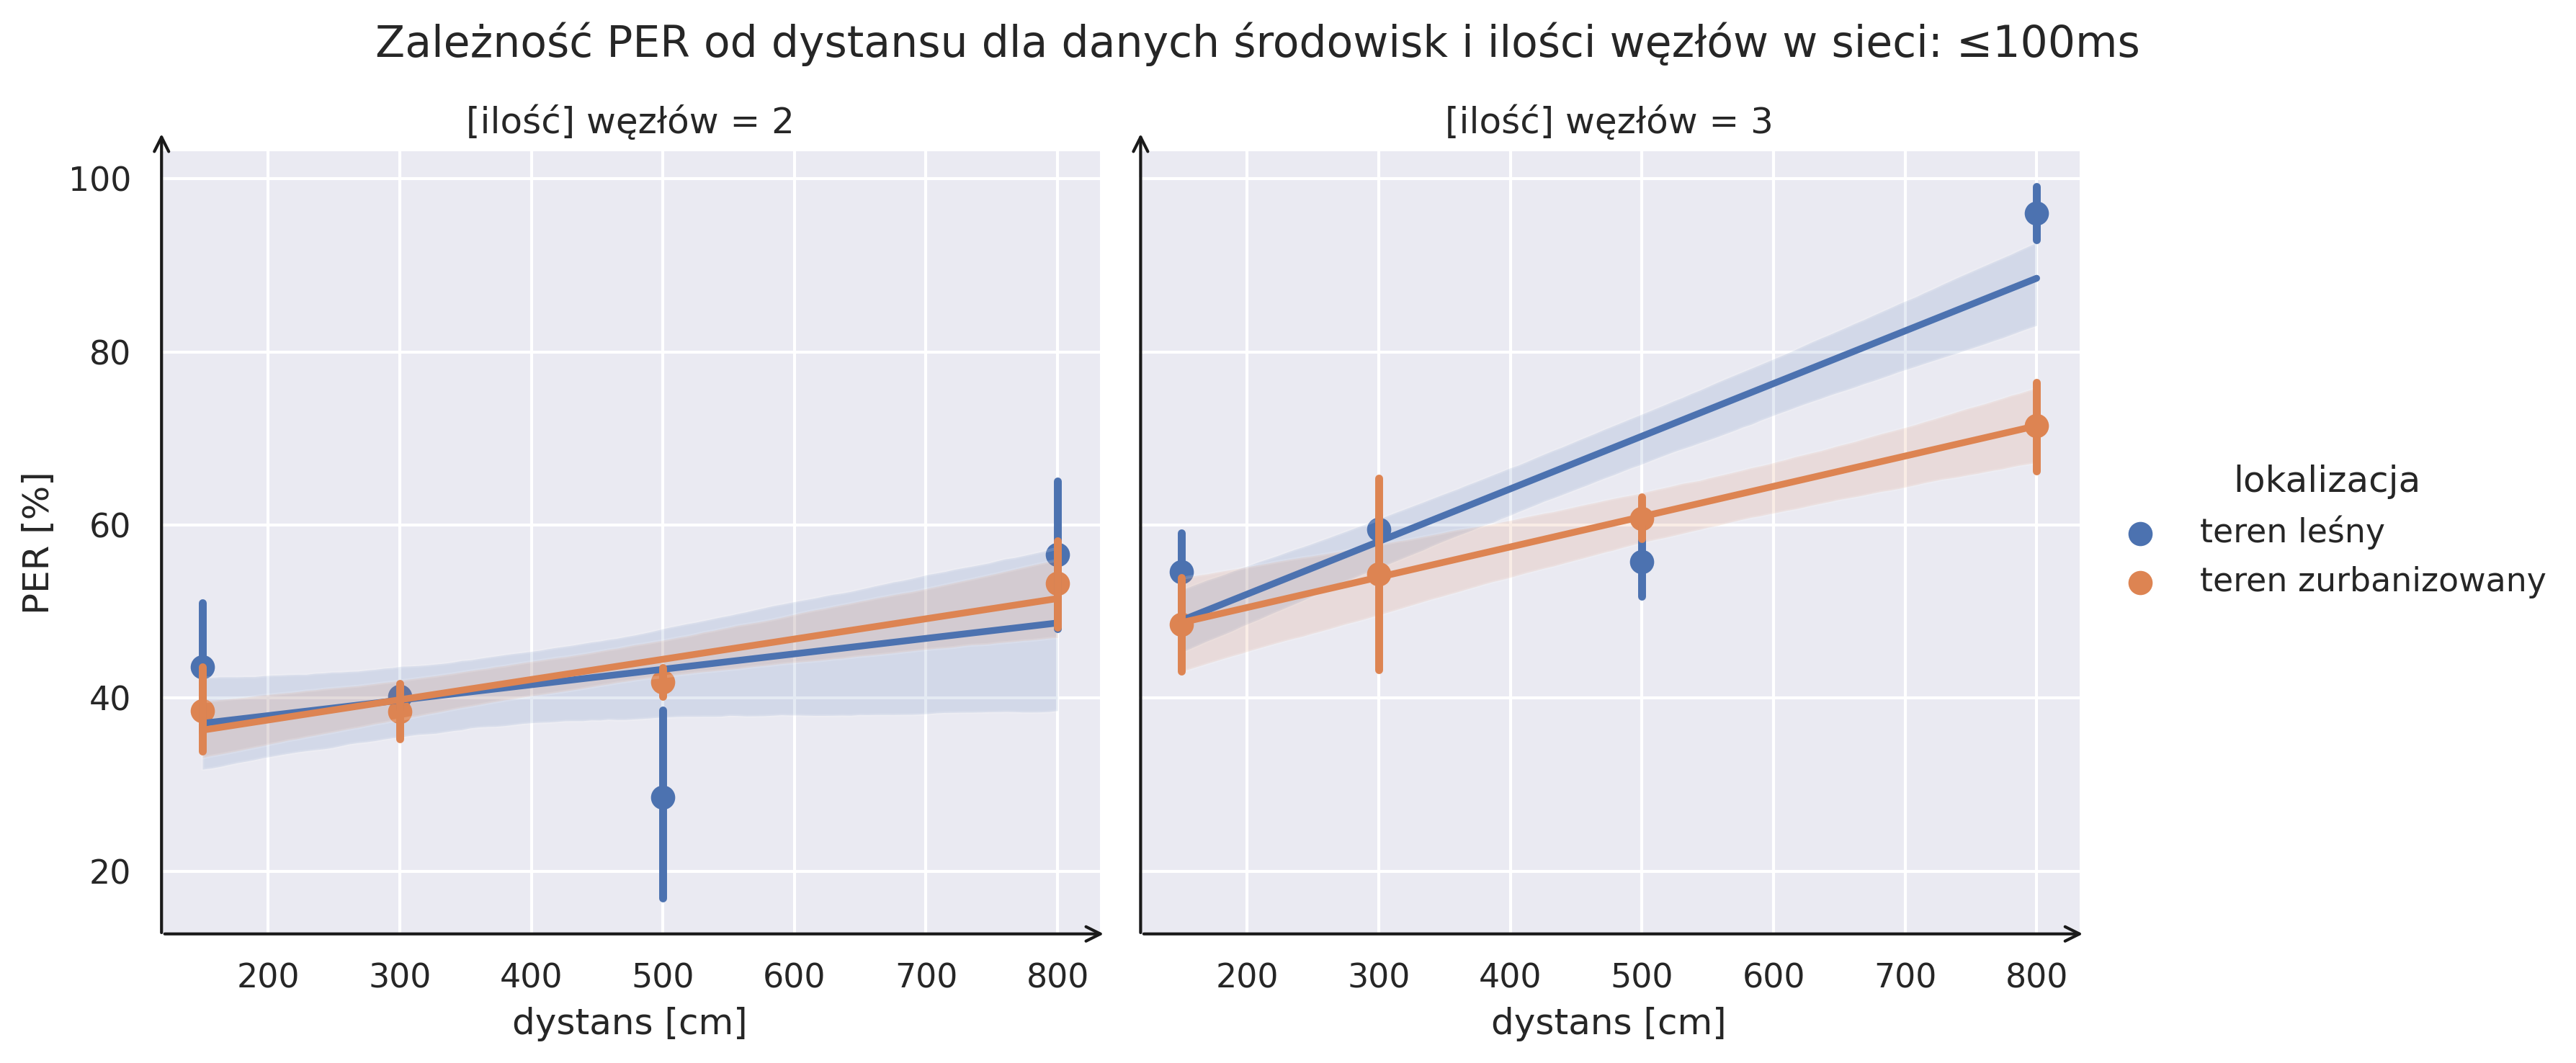
\includegraphics[width=0.99\linewidth]{per_to_distance_under_100ms_different_envs_and_nodes.png}
	\caption{Zależność \gls{PER} od dystansu dla zapytań o częstości $\leqslant$ 100ms w wybranych środowiskach i liczbę badanych węzłów}
	\label{rys:per_to_distance_under_100ms_different_envs_and_nodes}
\end{figure}

Znając charakterystykę łączności dla okresów poniżej 100 milisekund, weryfikuje się pozostałe wybrane częstości, zgodnie
z podanymi wartościami~\ref{items:ping_intervals}. Rysunek~\ref{rys:per_to_distance_over_100ms_different_envs_different_ping_interval}
prezentuje pozostałe interwały w zależności od dystansu i wybranych środowisk bez rozróżnienia na ilość węzłów w sieci.

Przeprowadzone pomiary w terenie leśnym wskazują charakterystykę połączenia zgodną z~intuicyjnymi przewidywaniami.
Na~początkowym dystansie 150cm nie obserwuje się problemów z łącznością. Wszystkie wysłane pakiety zostały
odebrane przez węzeł dalszy. Kolejny dystans wskazuje już na pewną utratę pakietów poniżej 20\%. Prawdopodobnym czynnikiem
jest pogoda lub ukształtowanie terenu leśnego. Co istotne, pomiary dla różnych interwałów odpytywań są zbliżone.
Sugerowałoby to brak wpływu częstości na \gls{PER}. Na pozostałych dystansach pomiarowych, wartości utraty pakietów
są do siebie wzajemnie zbliżone osiągając swoje maksimum na dystansie 21m - blisko 100\% zaginionych pakietów.

Charakterystyka łączności w terenie zurbanizowanym prezentuje się podobnie. Nie obserwuje się znaczącej utraty 
pakietów na względnie bliskich dystansach (150, 300 i 500cm). Wartość PER rośnie wraz ze wzrostem odległości
pomiędzy węzłami osiągając w swoim szczycie wartość ok. 40\%. Co istotne, linie aproksymacyjne są do siebie
zbliżone, ponownie sugerując brak korelacji pomiędzy częstością wysyłania komunikatów a~wartością PER.


\begin{figure}[!htb]
	\centering 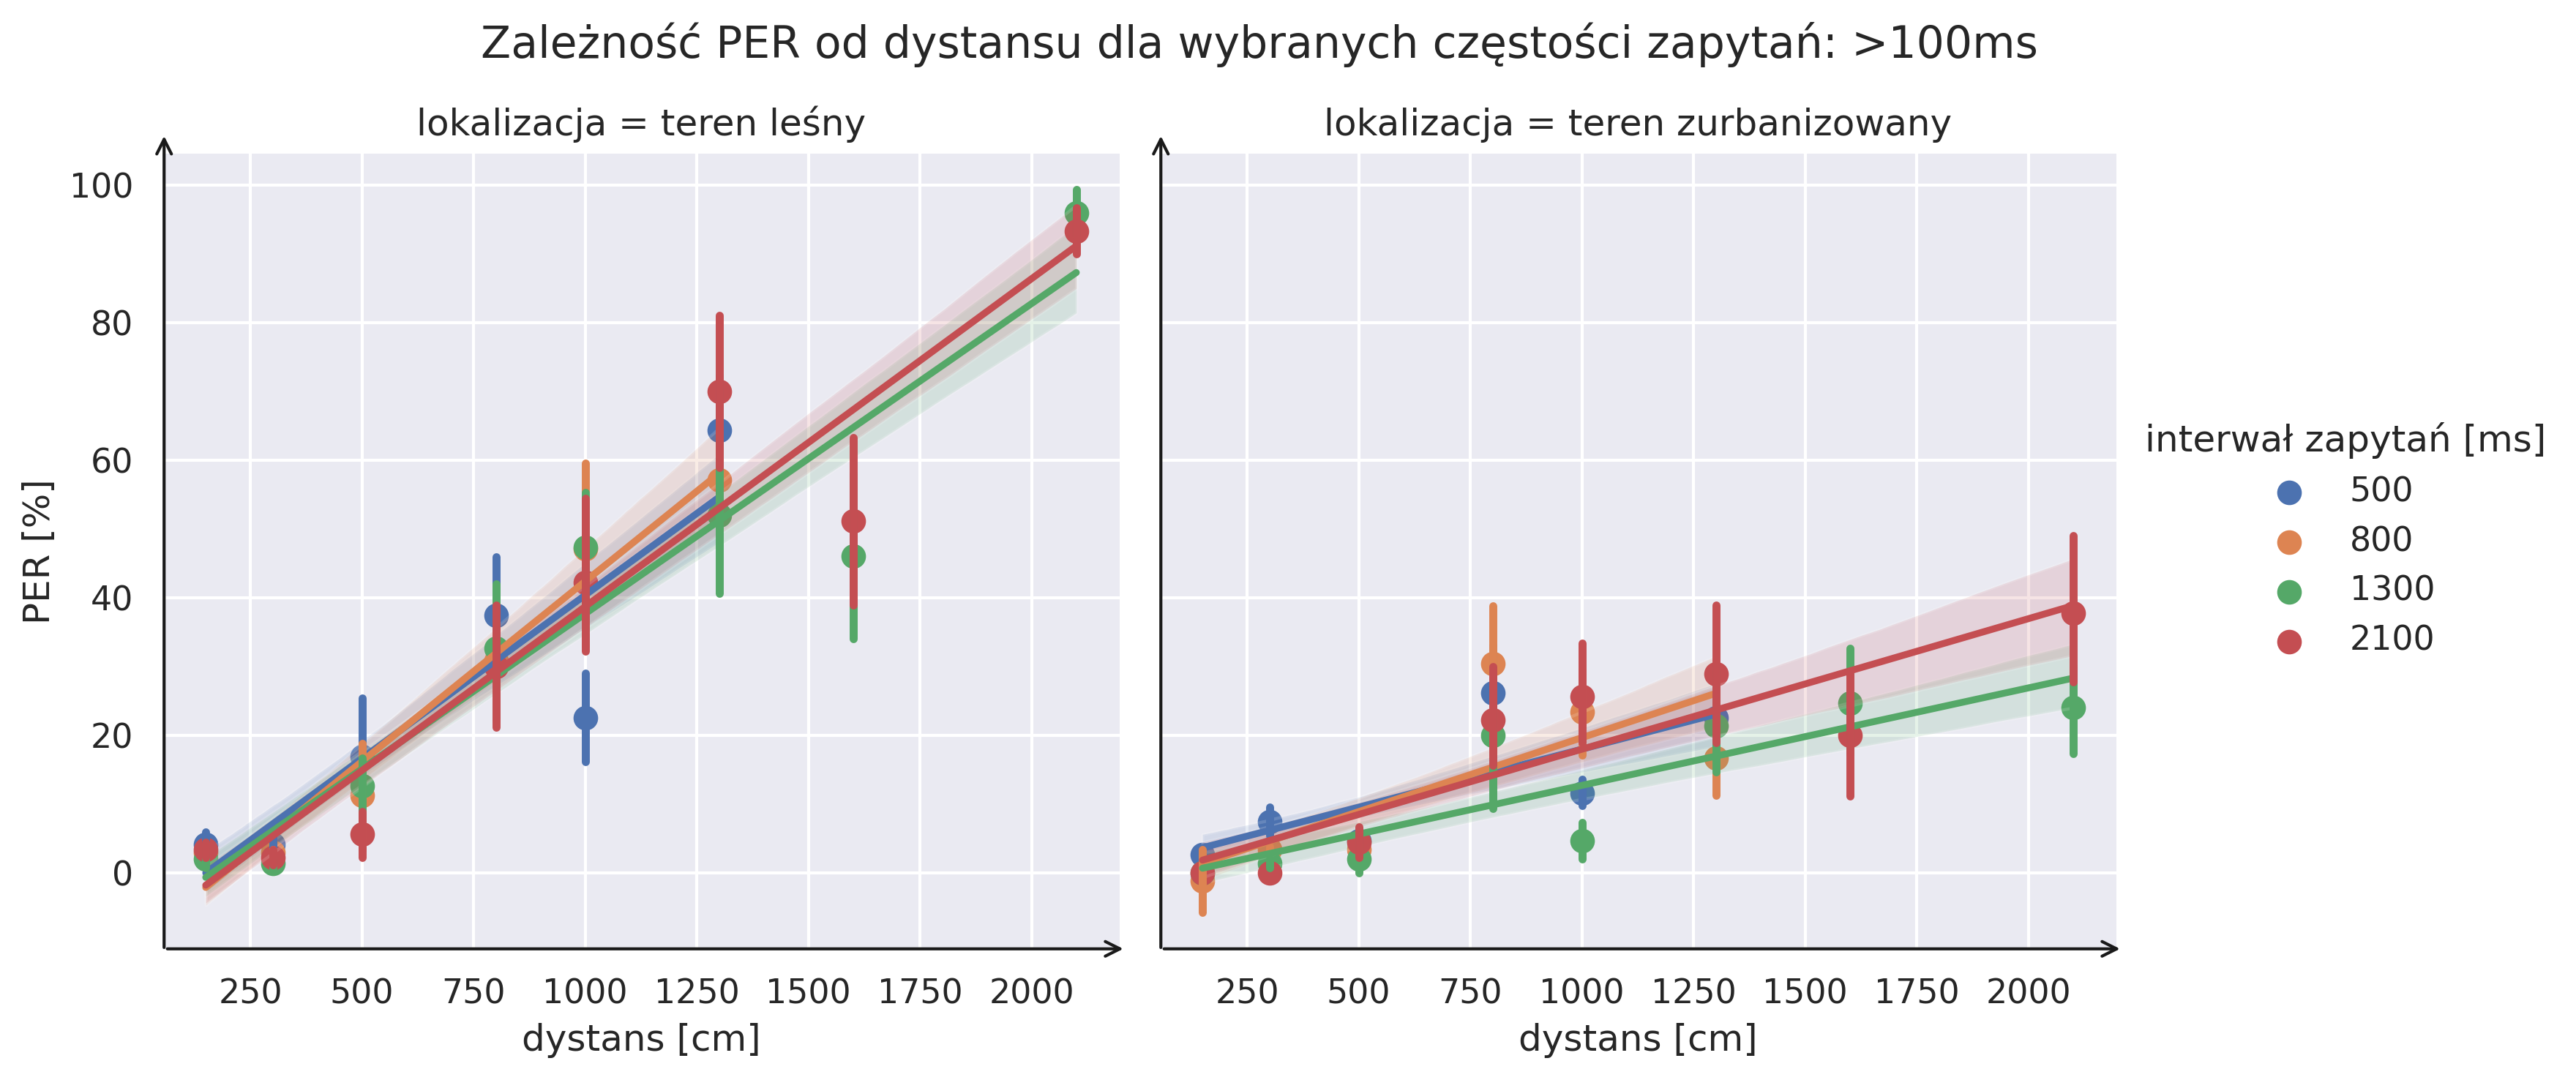
\includegraphics[width=0.99\linewidth]{per_to_distance_over_100ms_different_envs_different_ping_interval.png} 
	\caption{Zależność \gls{PER} od dystansu dla zapytań o częstości >100ms w wybranych środowiskach}
	\label{rys:per_to_distance_over_100ms_different_envs_different_ping_interval}
\end{figure}

Zależność pomiędzy PER a częstością odpytywań została zbadana wykorzystując narzędzia statystyczne. Traktując model
liniowy, jak sugerują zaprezentowane wykresy, tworzonych zgodnie z~metodą najmniejszych kwadratów wylicza się 
współczynnik determinacji dla następujących zmiennych niezależnych: dystans oraz PER. W~kolejnym kroku uwzględnia
się fakt wykorzystywania korelacji wielu zmiennych, dostosowując odpowiednio wartość.


\begin{table}[!ht]
\centering
	\begin{tabular}{p{4.5cm}|r|r}
	Środowisko              & $R^2$             & $R^2_{dostosowany}$\\\hline
	Teren leśny             & 0.04958           & 0.04272\\\hline
	Teren zurbanizowany     & 0.04887           & 0.04200\\\hline
	\end{tabular}
\caption{\label{tab:corr_between_ping_intervals}Współczynnik determinacji dla zależności interwału zapytań od dystansu i~PER w~wybranych środowiskach}
\end{table}

Ostatecznie, otrzymany współczynnik determinacji przyjmujący wartość $R^2=0,04-0,05$.  Istnieje 4\%-owy wpływ
interwału zapytań o częstościach większych niż 100 milisekund na ostateczny rezultat PER. Pozwala to
wykluczyć ten czynnik wykluczyć z dalszych rozważań uznając go za marginalny.

%%%%%%%%%%%%%%%%%%%%%%%%%%%%%%%%%%%%%%%%%%%%%%%%%%%%%%%%%%%%%%%%%%%%%%%%%%%%%%%%
%% SUBSECTION: Zależność \gls{PER} względem odległości między węzłami
%%%%%%%%%%%%%%%%%%%%%%%%%%%%%%%%%%%%%%%%%%%%%%%%%%%%%%%%%%%%%%%%%%%%%%%%%%%%%%%%
\subsection{Zależność PER względem odległości między węzłami}

Ustaliwszy brak (pomijalnie mały) wpływu częstości zapytań (dla częstości wartości >100ms), praca podejmuje dalszą prezentację
danych pod postacią zależności odległości na PER.

Rysunek~\ref{rys:per_to_distance_over_100ms} przedstawia zebrane dane zestawiając odległość i~ilość węzłów składających
się na sieć Mesh. Na początkowych dystansach PER ma wartość bliską bądź równą zeru. Wraz ze wzrostem odległości pomiędzy
węzłami, badany współczynnik rośnie, co jest zgodne z oczekiwaniami. Na dystansie 16m obserwuje się przełamanie
linii aproksymacji. Dodatkowy węzeł środkowy znacząco i pozytywnie wpływa na PER przy kolejnych odległościach
umożliwiając przekazywanie informacji w~sieci. PER w najdalszym punkcie pomiarowym osiąga wartości od ok.~60\% do 70\%.
Należy jednak mieć na uwadze, iż zestawienie nie rozróżnia środowiska w którym następowało zliczanie pakietów.


\begin{figure}[!htb]
	\centering 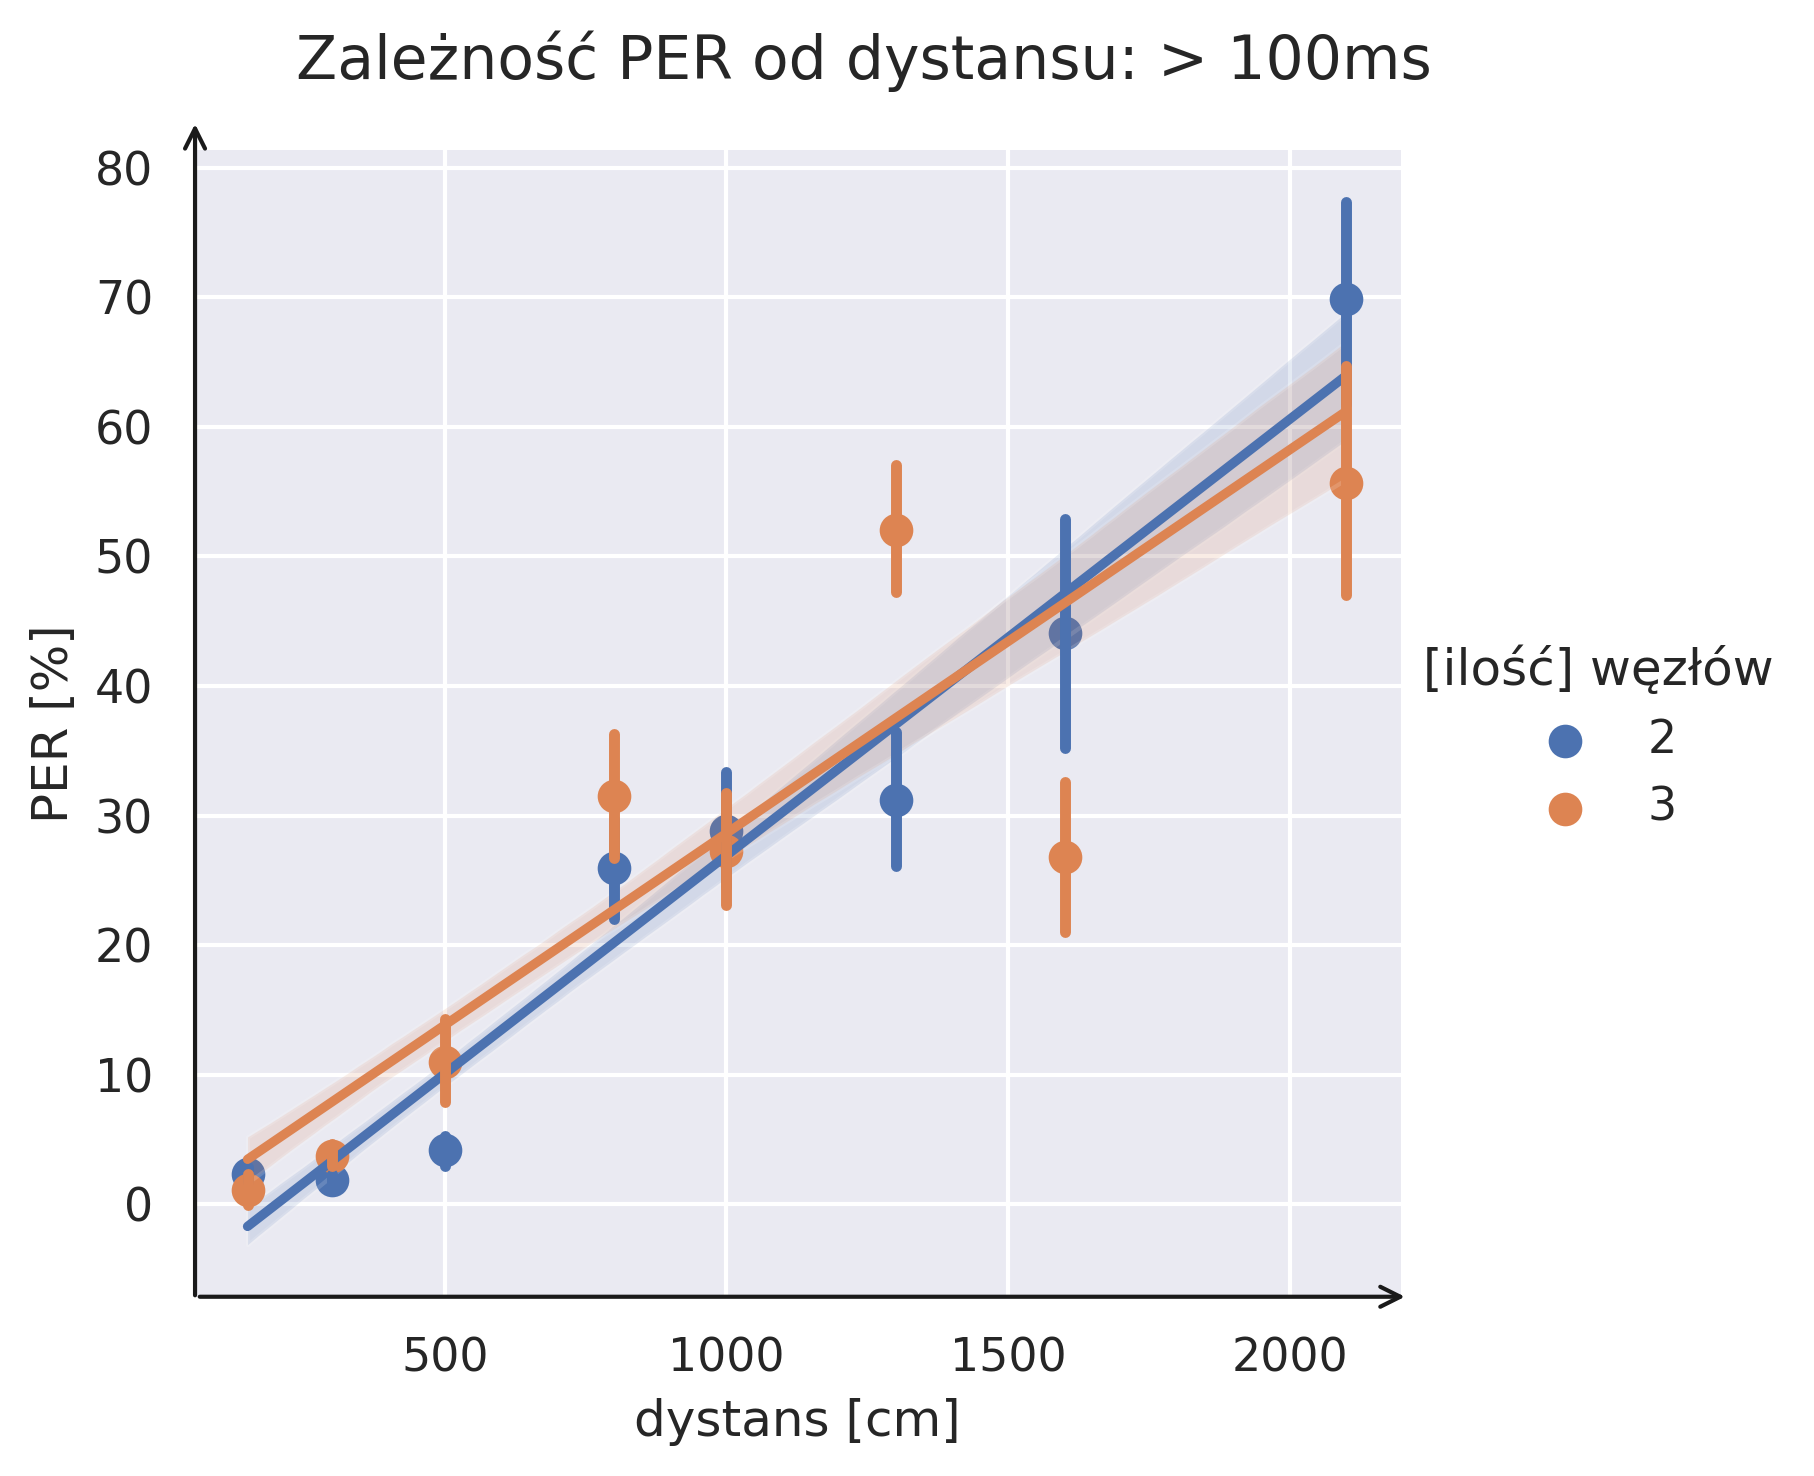
\includegraphics[width=0.618\linewidth]{per_to_distance_over_100ms.png}
	\caption{Zależność \gls{PER} od dystansu dla zapytań o częstości >100ms dla różnej liczby węzłów}
	\label{rys:per_to_distance_over_100ms}
\end{figure}

Rysunek~\ref{rys:per_to_distance_over_100ms_different_envs} uwzględnia wpływ środowiska na PER. Wykres zdecydowanie
wskazuje na różnicę pomiędzy terenem zurbanizowanym a terenem leśnym. Na początkowych dystansach PER jest zbliżone
niezależnie od odległości międzywęzłowych. Znaczące różnice w pomiarach, a dzięki temu również względem linii aproksymacyjnej,
występują już na dystansie 5m. PER w przypadku miejskim jest bliskie zera, gdzie analogiczne pomiary w środowisku
leśnym sugerują piętnastoprocentowy poziom zgubionych pakietów. Wraz ze wzrostem dystansu, wartość PER wzrasta.
Niemniej jednak nachylenie linii wskazuje na zdecydowanie wolniejsze narastanie utraty danych podczas transmisji
bezprzewodowej dla przypadku miejskiego. Na maksymalnym dystansie międzywęzłowym wynoszącym 21m, PER
przybiera wartość ok. 30\%. W analogicznym przypadku dla środowiska leśnego następuje niemal całkowita utrata
transmisji.

\begin{figure}[!htb]
	\centering 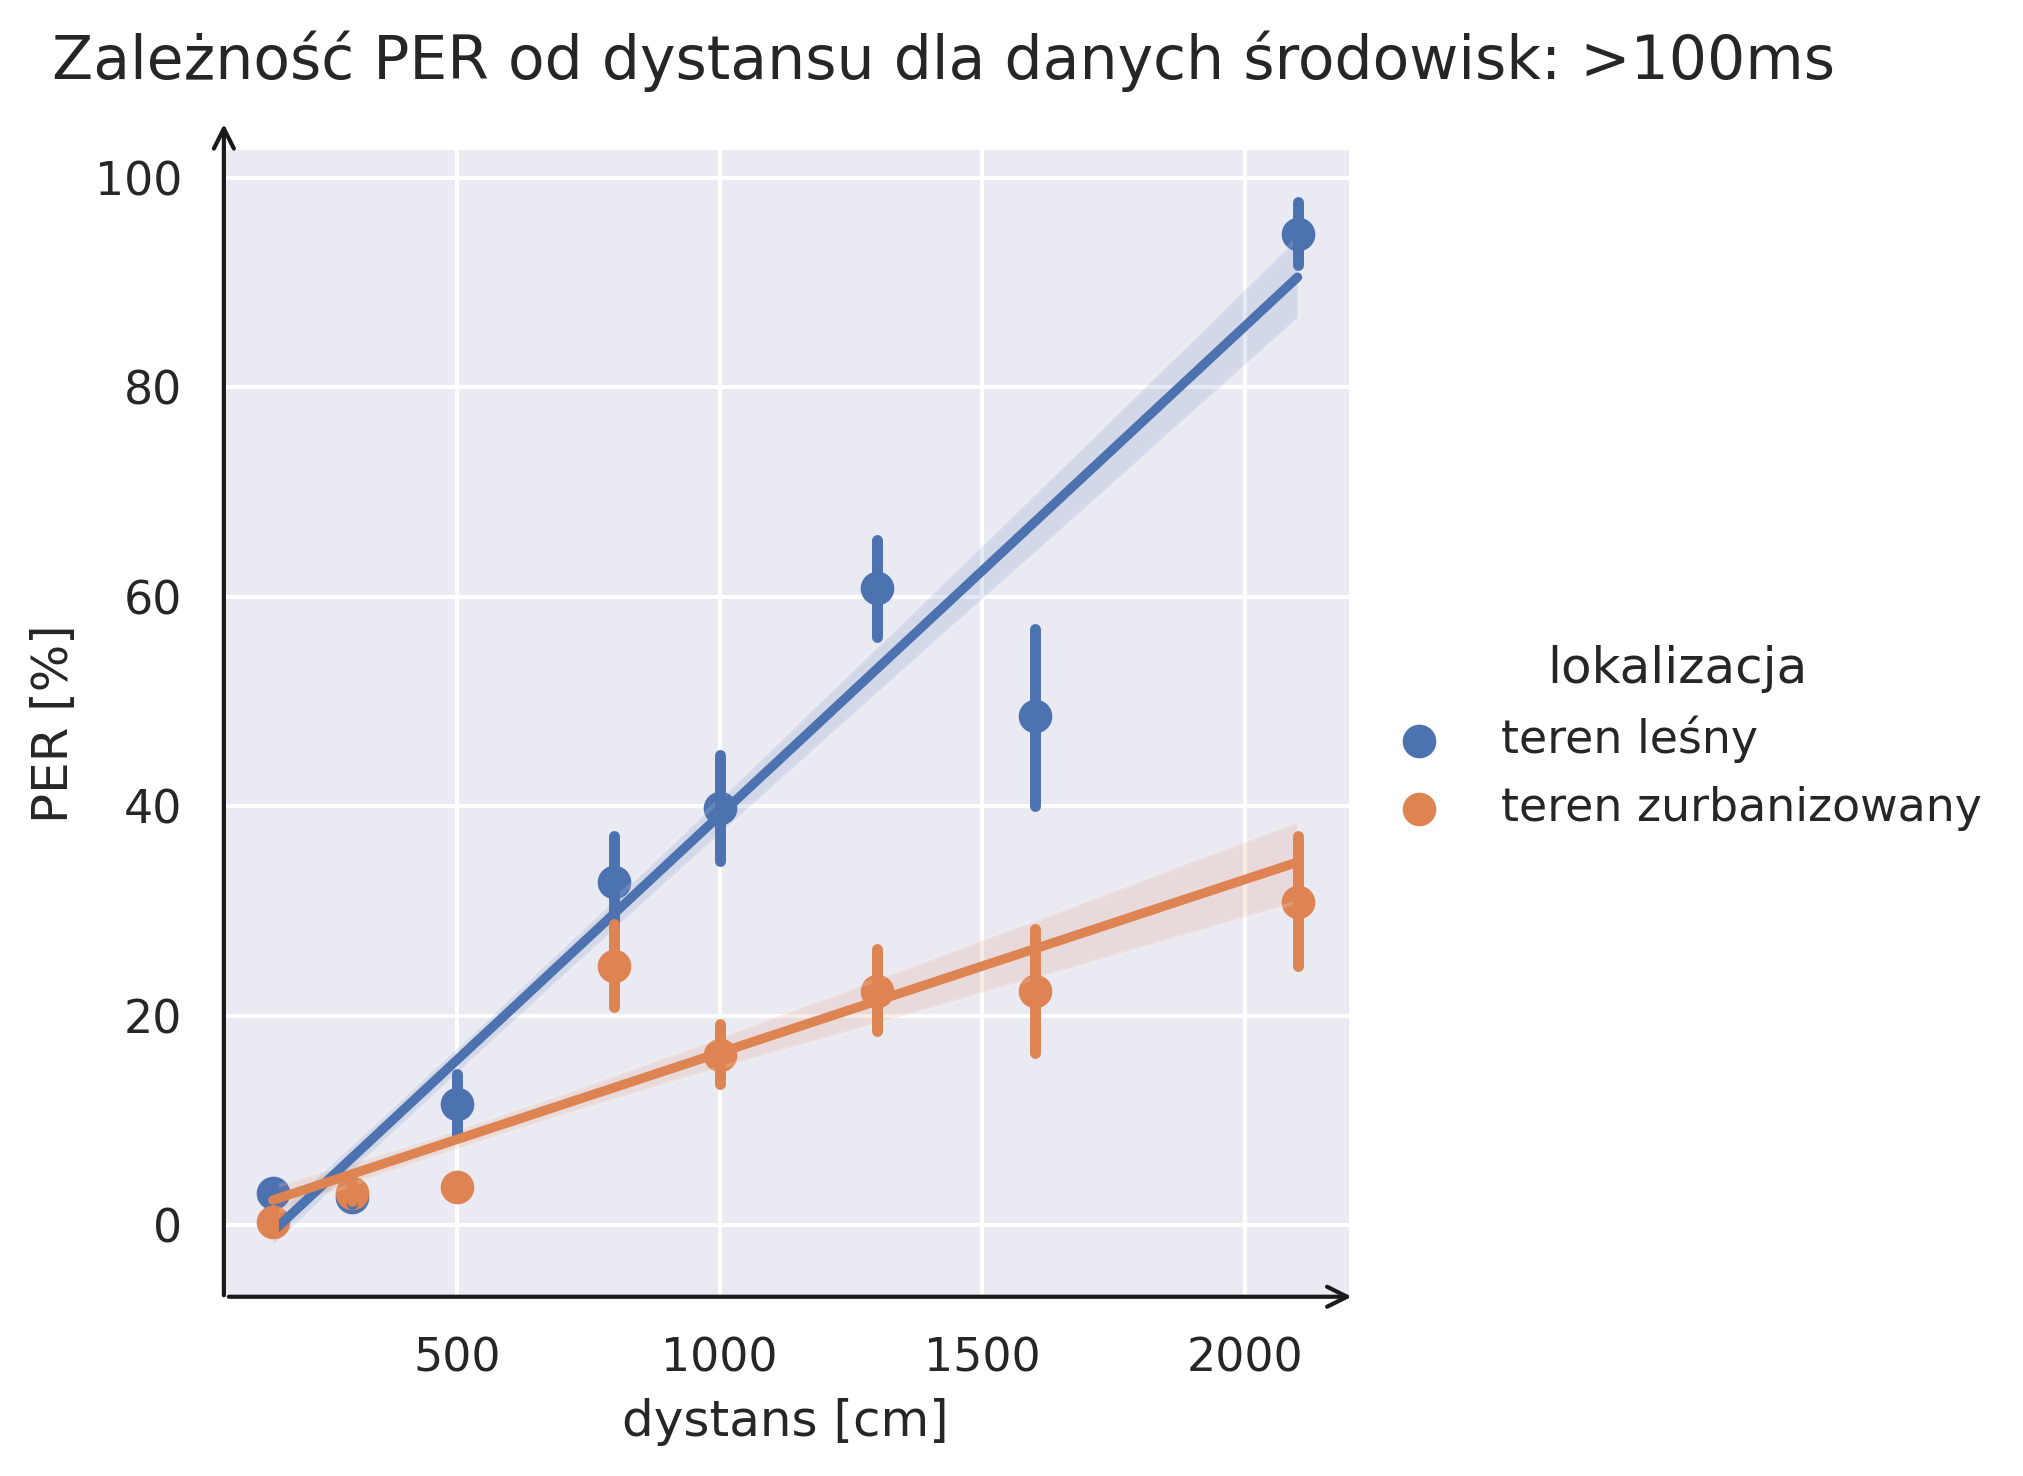
\includegraphics[width=0.618\linewidth]{per_to_distance_over_100ms_different_envs.png} 
	\caption{Zależność \gls{PER} od dystansu dla zapytań o częstości >100ms w wybranych środowiskach bez rozróżnienia na liczbę węzłów}
	\label{rys:per_to_distance_over_100ms_different_envs}
\end{figure}

Ostatnia prezentowana zależność ukazana jest na Rysunku~\ref{rys:per_to_distance_over_100ms_different_envs_and_nodes}.
Przedstawia on zależność PER od dystansu dla wybranych środowisk i liczby węzłów.

\begin{figure}[!htb]
	\centering 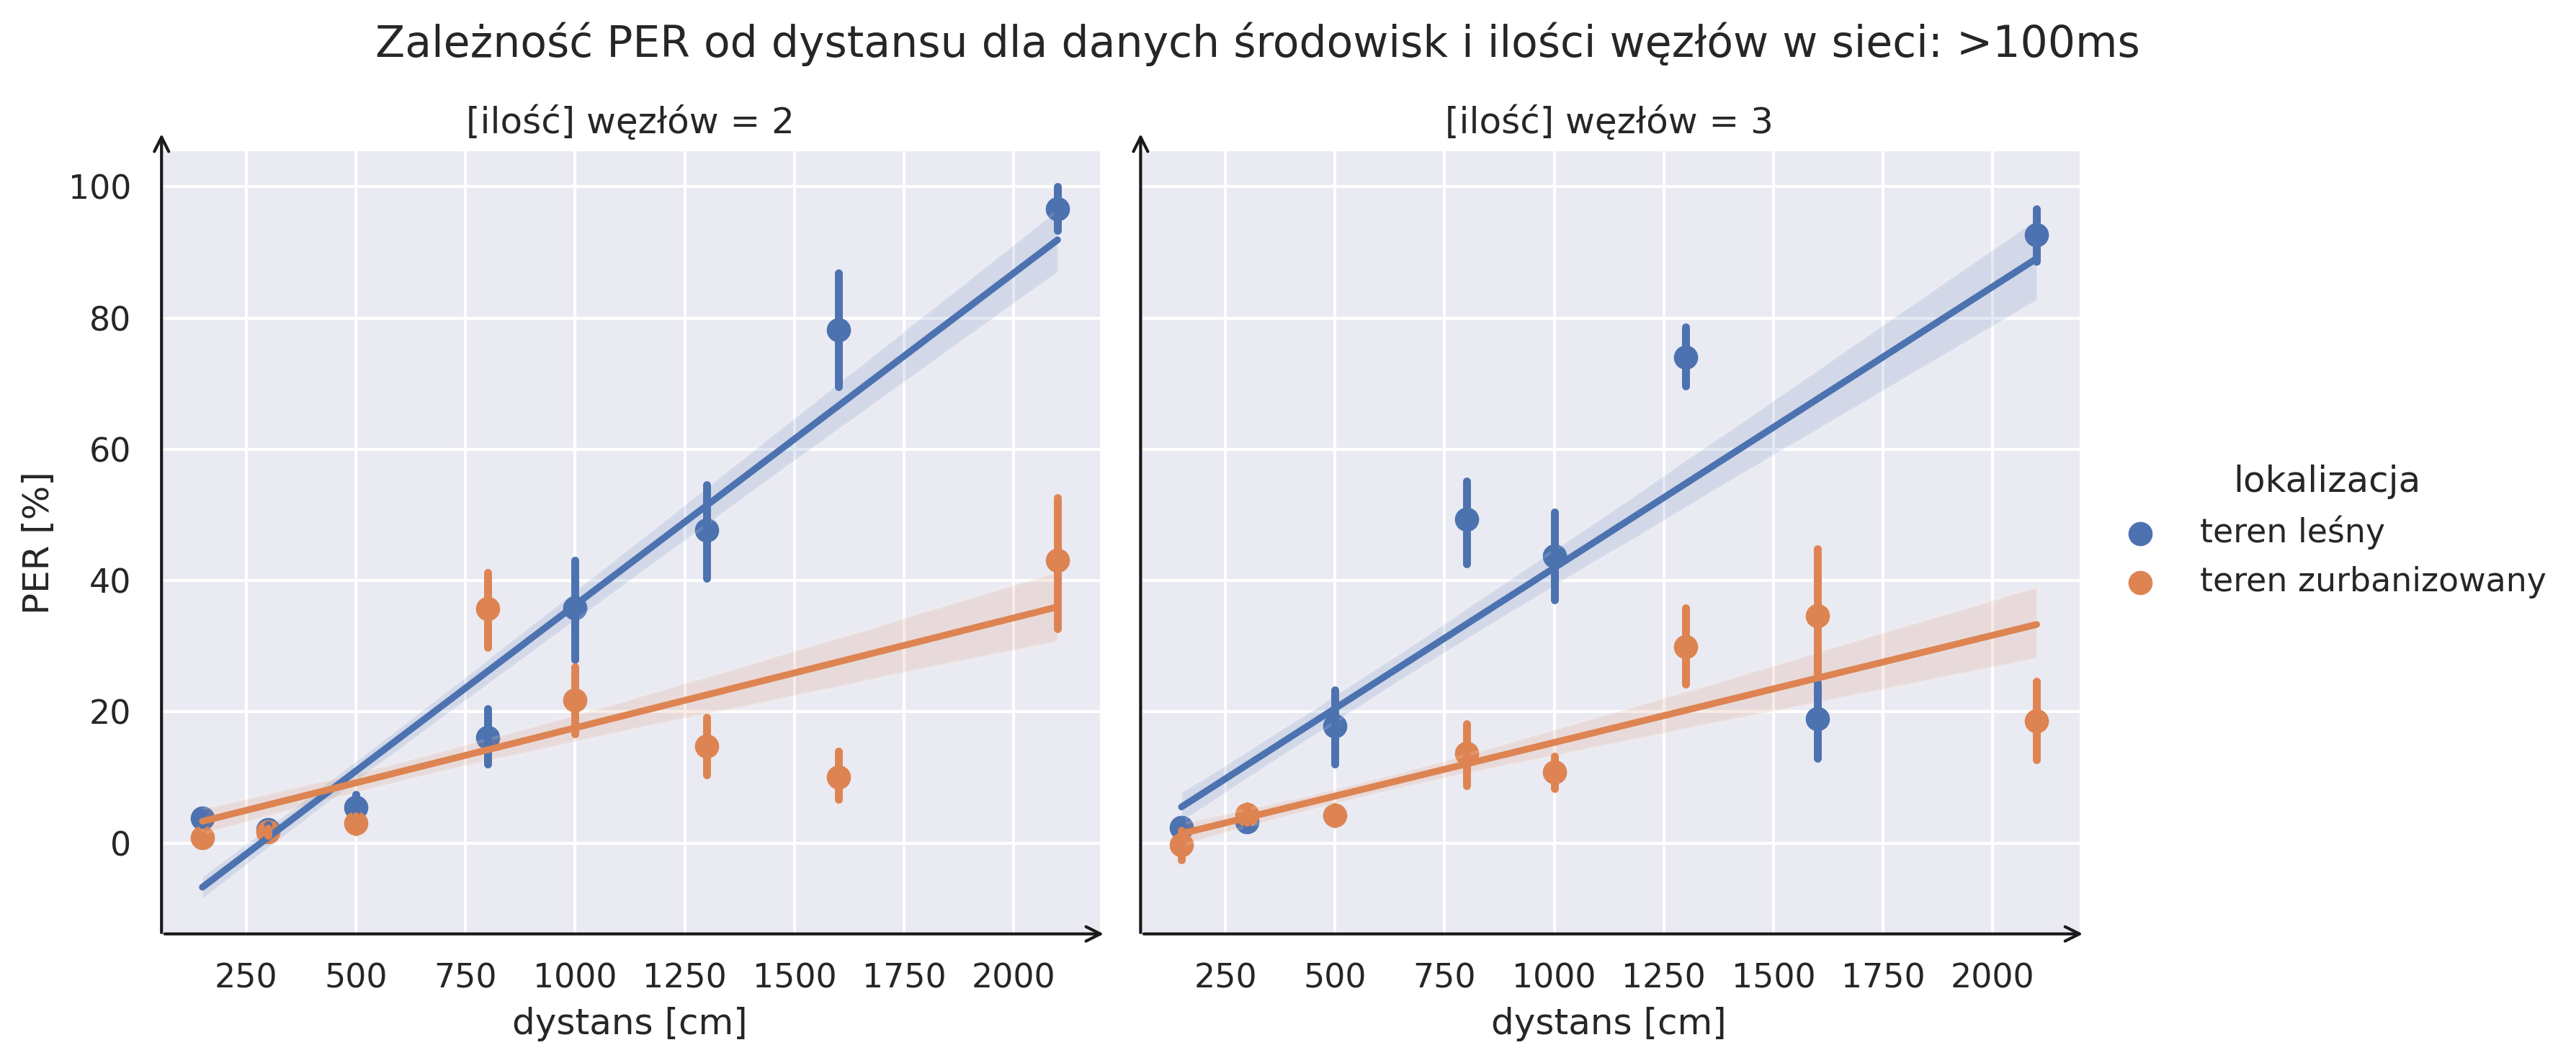
\includegraphics[width=0.99\linewidth]{per_to_distance_over_100ms_different_envs_and_nodes.png}
	\caption{Zależność \gls{PER} od dystansu dla zapytań o częstości >100ms w wybranych środowiskach i liczbę badanych węzłów}
	\label{rys:per_to_distance_over_100ms_different_envs_and_nodes}
\end{figure}



